\documentclass[journal,twoside,web]{ieeecolor}

%cụm lệnh viết tiến việt
\usepackage{vntex}
\newcommand{\tv}[1]{{\fontfamily{ptm}\selectfont #1}}

\usepackage[final]{changes}% tăt thay đổi khi dùng final
% \usepackage[markup=strikeout]{changes}
\usepackage{tabularx}
% Chuyển tất cả nội dung bị xóa/thay bằng màu đỏ
\usepackage[hidelinks]{hyperref} %tùy chọn Ẩn màu (text giữ nguyên màu đen),
\usepackage[ruled,vlined]{algorithm2e}
\usepackage{threeparttable}
\usepackage{jsen}

\usepackage{cite}
\usepackage[table]{xcolor}
\usepackage{amsmath,amssymb,amsfonts}
% \usepackage{algorithmic}
\usepackage{graphicx}
\usepackage{textcomp}
\usepackage{wrapfig}
\usepackage{array,multirow,multicol,makecell}%
% \usepackage{amsthm}%
\usepackage{mathrsfs}%
% \usepackage[title]{appendix}%
\usepackage{textcomp}%
\usepackage{manyfoot}%
\usepackage{booktabs}%
\usepackage{hyperref}
% \usepackage{algorithm}%
% \usepackage{algorithmicx}%
\usepackage{algpseudocode}%
\usepackage{listings}%
\usepackage{placeins}
\usepackage{ragged2e}
\usepackage{footnote}
\usepackage{float}
\usepackage{placeins}
\usepackage{lipsum} % (Tùy chọn) Để tạo văn bản giả lập
\usepackage{url}
\renewcommand{\UrlFont}{\normalfont}
\def\BibTeX{{\rm B\kern-.05em{\sc i\kern-.025em b}\kern-.08em
    T\kern-.1667em\lower.7ex\hbox{E}\kern-.125emX}}
\markboth{\journalname, VOL. XX, NO. XX, XXXX 2025}
{To-Hieu Dao \MakeLowercase{\textit{et al.}}: Preparation of Papers for IEEE TRANSACTIONS and JOURNALS (May 2025)}
\definecolor{abstractbg}{rgb}{0.89804,0.94510,0.83137}
\setlength{\fboxrule}{0pt}
\setlength{\fboxsep}{0pt}

\begin{document}
\title{RFAR: A Real-time Firefighter Activity Recognition System Using Wearable Accelerometer}
\author{To-Hieu Dao, Duc-Nghia Tran, Viet-Hoan Bui, Van Son Nguyen, Dang Khanh Hoa, Pham Van Thanh and Duc-Tan Tran, \IEEEmembership{Member, IEEE}
\thanks{To-Hieu Dao, Viet-Hoan Bui, and Duc-Tan Tran are with the Phenikaa School of Engineering, Phenikaa University, Hanoi, Vietnam. In addition, To-Hieu Dao is a Ph.D. student at the Graduate University of Science and Technology, VAST. Email: \{hieu.daoto,tan.tranduc\}@phenikaa-uni.edu.vn, 21011096@st.phenikaa-uni.edu.vn.}
\thanks{Duc-Nghia Tran is with the Institute of Information Technology, VAST, Hanoi, Vietnam. Email: nghiatd@ioit.ac.vn. }
\thanks{Van Son Nguyen and Dang Khanh Hoa are with the Hanoi Open University, Vietnam. Email: \{sonnv, dkhoa2\}@hou.edu.vn.}
\thanks{Pham Van Thanh is with the University of Fire Prevention and Fighting, Hanoi, Vietnam. E-mail: phamvanthanh1209@gmail.com.}
\thanks{Corresponding: dkhoa2@hou.edu.vn (Dang Khanh Hoa).}}

\IEEEtitleabstractindextext{%
\fcolorbox{abstractbg}{abstractbg}{%
\begin{minipage}{\textwidth}%
% \begin{wrapfigure}[12]{r}{3in}%
% 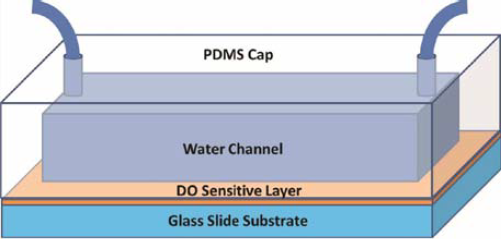
\includegraphics[width=3in]{jsenga.png}%
% \end{wrapfigure}%
\begin{abstract}
Human Activity Recognition (HAR) presents significant challenges. Although HAR is mainly used for elderly care, it holds significant potential for supporting firefighter operations. The main challenge of HAR is the recognition of complex actions and continuous transitions from real-time data. This study proposes a Real-time Firefighter Activity Recognition (RFAR) system that accurately recognizes eleven activities. The proposed system is based on a wearable device with an integrated accelerometer, ensuring compactness and energy efficiency. It can optimize parameters for deploying the random forest (RF) model on performance-constrained microcontrollers. A new data processing pipeline that integrates a sliding window technique with an abnormality index detection technique is proposed. This method achieves an F1-score of 96.1~\% on a private dataset. Real-time experiments with a waist-mounted accelerometer achieved an F1-score of 96.2~\% in rescue simulations conducted by volunteers at a firefighting training facility in Vietnam. To validate, the method is performed on three public datasets: achieving an F1-score of 96.6~\% on SFDLA, 96.6~\% on MobiFall, and 78.2~\% on UniMiB-SHAR. Another contribution of this study is the development of a specialized dataset that comprehensively represents fundamental and unique firefighter activities in realistic scenarios.
\end{abstract}

\begin{IEEEkeywords}
Firefighter, activity, recognition, RFAR, wearable device, real-time, accelerometer.
\end{IEEEkeywords}
\end{minipage}}}

\maketitle
\section{Introduction}
\label{sec:introduction}

Rapid urbanization and the gradual deterioration of infrastructure have contributed to increased latent risks of fire and explosion in both residential and industrial zones \cite{Clarke2021firefighter}.
Uncontrolled construction activities and poor management have left many buildings vulnerable to safety hazards \cite{Fialho_Fire2024}. Meanwhile, many local fire protection systems have become outdated or insufficient to meet current operational demands \cite{Rosengren_FIRE2014}. These factors have led to a rise in the number of fire incidents, which tend to exhibit greater severity \cite{Fialho_Fire2024}.

Firefighters play a central role in emergency response operations and frequently face potential hazards \cite{FirefighterImportant2022}.
Common hazards include extreme heat \cite{Firefighterhealthcare2024}, toxic gases \cite{Firefighter_toxis}, confined spaces \cite{Firefighter_limited2019}, and the potential for structural collapse \cite{Firefigter_toxis_2016}. In the United States, a total of 23,075 rescue workers were injured according to a report on firefighter fatalities during 2018~--~2020\footnotemark[1] period. The majority of these injuries, accounting for 87~\%, occurred during structural fires, where the likelihood of permanent injuries is ten times higher than in non-structural fires. The NFPA statistics\footnotemark[2] estimated 63,175 injuries, with 89 on-duty fatalities reported in 2023. Fire suppression activities posed the highest risk, accounting for approximately 18,875 cases. A significant challenge faced by firefighters is the lack of tools and solutions to support them in their duties \cite{carmona2024firefighters,FirefighterClothing2022,Thanhfire2019,Firefighter_Falling_2023}.

\footnotetext[1]{\url{https://www.usfa.fema.gov/statistics/} (Accessed: 12:00 25/01/2025).}
\footnotetext[2]{\url{https://www.nfpa.org/} (Accessed: 8:00 25/01/2025).}

The application of science and technology significantly enhances firefighter safety \cite{Firefighter_limited2019,FirefighterImportant2022,carmona2024firefighters}. Recent research has focused on three main areas of improvement: upgrading the protective gear to mitigate the effects of heat and toxic chemicals \cite{FirefighterClothing2022, Firefighter_toxis}; monitoring psychological and health status under high-stress working conditions \cite{Firefighterhealthcare2024, Rosengren_FIRE2014}; and developing on-site monitoring and communication systems to assist decision-making \cite{FirefighterImportant2022,Thanhfire2019, Firefighter_Falling_2023}.
Among these, communication systems between command units and frontline firefighters are critical in maintaining continuous communication for operational coordination \cite{Rosing04032022, Takacs2022}.

 
Monitoring of firefighters' performance and their communication with commanders are vital for rescue personnel's timely response and risk mitigation to  \cite{Firefighter_limited2019,FirefighterImportant2022}. However, traditional communication methods such as two-way radios often provide fragmented information and lack the ability to monitor the real-time status of individual personnel \cite{Clifford2021}. This significantly hampers rescue coordination, especially when the location or condition of a firefighter cannot be determined—such as in cases of unconsciousness or immobility \cite{Zhang2024}. Delayed responses in such situations may lead to severe consequences \cite{carmona2024firefighters, Waring2024, Tamrakar2020}.

The lack of accurate and continuous information on each firefighter’s position and conditions poses major challenges for command and rescue coordination \cite{RF_ForestFires2024,Firefighter_Falling_2023,Firefighterhealthcare2024}. HAR for firefighters, combined with location information, is a potential solution that provides objective and continuous data, supporting timely decision-making \cite{Accelerometerlocation2021}. HAR is commonly approached through two primary methods: computer vision \cite{HARvision2020} and wearable sensor signals \cite{HongNhung2023}. However, Dang \cite{HARvision2020} identified the main drawbacks of vision-based activity recognition methods, including sensitivity to environmental conditions, complex data processing requirements, and privacy concerns due to continuous recording. In contrast, wearable sensors are highly appreciated for their outstanding advantages, such as compact size, low cost, and the ability to quickly detect kinematic changes \cite{Accelerometer2021,DaoHieu2022,ViManhTuyen2024,HongNhung2023,Thu2022,AccelerometerHAR2023,accelerometer_error2024,Thanhfire2019,Chai2021,CHAI_FIRE2024}. 

Tab.~\ref{Table_firemanActivityRecognition} provides an overview of recent studies in HAR, utilizing wearable devices equipped with accelerometers. They are typically placed at positions such as the waist \cite{Thu2022,Elder_Falling_2019}, wrist \cite{Lu2020}, or thigh \cite{Thanhfire2019} to collect activity data. Many studies have integrated accelerometers with other sensors, such as gyroscopes \cite{DaoHieu2022}, carbon monoxide sensors \cite{Dang2022}, or 9-axis inertial sensors \cite{Chai2021} to enhance the detection of complex movements. Additionally, electromyography sensors \cite{CHAI_FIRE2024} have been used to capture detailed muscle signals.

Accelerometer-based HAR is commonly used in health monitoring \cite{HumanActivityRecognition2022,Wang2018,MobiFall_Yi_2024, HAR_DCT_deeplearning2023, Fall_Elder2019, Fall_Elder2022, Elder_Falling_2019, SFDLAdataset2016}, but it also holds potential for real-time activity tracking and incident detection in firefighters \cite{Xu_fire2020,wearableFirefirefighter2015,wearableFirefirefighter2018}. Most studies primarily focus on distinguishing fall situations \cite{ Chai2021,CHAI_FIRE2024, Thanhfire2019, Rosengren_FIRE2014}, with little attention given to specific firefighter activities \cite{Chai2021,CHAI_FIRE2024} such as crawling, slithering. These activities are performed in harsh environments with high temperatures, thick smoke, and confined spaces \cite{Shah2024}, making recognition challenging. The main challenges stem from the similarity of postures, the difficulty in controlling sensor data, and their continuous real-time transitions. Nevertheless, recent studies have applied deep learning (DL) \cite{HAR_DCT_deeplearning2023,CHAI_FIRE2024,DL2021_HAR_wearable,HAR_DL_sensor2023} to improve recognition accuracy. These approaches typically require high computational resources, making it challenging to implement them on microcontrollers with limited memory, processing speed, and energy capacity. High energy consumption shortens operational time, necessitates larger batteries, and limits the design of compact wearable devices for firefighters. To address this, adopting lightweight machine learning (ML) models deployable on microcontrollers offers a practical solution for optimizing resources while maintaining a balance between accuracy, processing speed, and power efficiency. 

\begin{table}[h!]
    \caption{Overview of HAR using wearable devices.}
    \label{Table_firemanActivityRecognition}
    \footnotesize
    \renewcommand{\arraystretch}{1.2} % Điều chỉnh khoảng cách giữa các hàng
    \resizebox{\columnwidth}{!}{ % Co bảng theo chiều rộng của cột
\begin{tabular}{
    >{\centering\arraybackslash}m{0.05\linewidth} % Căn giữa cả theo chiều ngang và dọc
    >{\RaggedRight\arraybackslash}m{0.54\linewidth} % Căn trái theo chiều ngang và giữa theo chiều dọc
    >{\RaggedRight\arraybackslash}m{0.12\linewidth} % Tương tự
    >{\RaggedRight\arraybackslash}m{0.225\linewidth} % Tương tự
}
        \noalign{\hrule height 1.2pt} % Dòng kẻ tiêu đề đậm hơn
      \rowcolor{gray!20}\textbf{Year} & \textbf{Dataset} & \textbf{Research object} & \textbf{Methods} \\
        \noalign{\hrule height 1.2pt} % Dòng kẻ tiêu đề đậm hơn
 \multirow{1}{*}{2024} & Accelerometer ; UniMiB (50~Hz), WISDM (20~Hz), UCI (50~Hz); body: front pocket. & Human, activity & CLS-CNN-ResNest \cite{HAR_CNN_2024}\\

        \hline
        
        \multirow{1}{*}{2024} & Fusion sensors; 100~Hz; 18 volunteers; body: arm, upper arm, calf; 8 activities & Firefighter, activity & Hybrid ML \cite{CHAI_FIRE2024}\\
        \hline
        
        \multirow{1}{*}{2023} & Accelerometer; Opportuni (30~Hz), UniMiB (50~Hz), UR Fall (256~Hz), UCI (50~Hz); body: front pocket. & Human, activity  & CNN-DCT, ResNet-DCT \cite{HAR_DCT_deeplearning2023}\\

        \hline
        
        \multirow{1}{*}{2022} & Accelerometer, CO; 100~Hz; 8 volunteers; body: waist; 2 activities & Firefighter, falling & Fall detection \cite{Dang2022}\\
        \hline
        \multirow{1}{*}{2021} & 9-axis\footnotemark[1], 15~Hz; 10 volunteers; body: chest, elbow, waist, thigh, ankle; 2 activities& Firefighter, falling& LSTM \cite{Chai2021}\\
        \hline
        \multirow{1}{*}{2021} & Accelerometer; WISDM (20~Hz), PAMAP2 (33.33~Hz), UniMiB (50~Hz), UCI (50~Hz); body: front pocket. & Human, activity & HARMamba \cite{HAR1_DL_2021}\\
        \hline
        \multirow{1}{*}{2020} & Accelerometer; 50~Hz; 21 volunteers body: wrist; 6 activities & Human, activity & GBDT, RF, KNN, SVM \cite{Lu2020}\\
        \hline
        \multirow{1}{*}{2019} & 9-axis, CO; barometer; 100~Hz; 6 volunteers; body: front trouser, pocket; 2 activities& Firefighter, falling & Fall detection \cite{Thanhfire2019}\\

        \hline
        \multirow{1}{*}{2019} & Accelerometer; 50~Hz; 16 volunteers; body: waist; 2 activities& Elder, falling & Fall detection \cite{Elder_Falling_2019}\\

        \hline
        \multirow{1}{*}{2016} & On-body radio frequency, doppler; 20~Hz; body: chest, forehead, right wrist, right ankle; 7 activities& Firefighter, activity  & SVM \cite{Geng2016}\\
        \noalign{\hrule height 1.2pt} % Dòng kẻ cuối cùng đậm hơn
    \end{tabular}}
\end{table}
\footnotetext[1]{9-axis: accelerometer, gyroscope, magnetic.}

This study makes the following contributions:
\begin{itemize}
\item First, a dedicated dataset was constructed to simulate firefighter activities during rescue training drills, aiming to supplement the gaps in existing public datasets.

\item Second, this study developed a new signal processing pipeline that combines a sliding window technique with abnormality index detection to enhance the quality of activity information at each stage. This pipeline thoroughly considers the transition process between actions and is suitable for deployment on resource-constrained microcontrollers. This aspect has received little attention in previous studies, which primarily focused on homogeneous and continuous actions.

\item Third, this study introduces the RFAR system, which employs a wearable device with a waist-mounted accelerometer to recognize eleven firefighter-specific activities, including walking (WA), standing (ST), lying (LY), sitting (SI), jogging (JO), walkstoop (WS), crawling (CR), slithering (SL), falling (FA), downstairs (DS), upstairs (US). The system is implemented on a low-power microcontroller using an RF model and a feature set, both of which have been optimized. It achieves high accuracy while keeping the model size under 1~MB, making it suitable for deployment on resource-constrained embedded platforms.

\item Fourth, the developed wearable device is lightweight (under 200 grams), enables continuous operation for up to 24 hours, and is designed for portability and comfort of users on the scene. The system was evaluated on volunteers from Phenikaa University and the University of Fire Prevention and Fighting in Vietnam, showing consistent results with over 96~\% F1-score and 99~\% accuracy in realistic simulated rescue scenarios. The system was also tested on public datasets including SFDLA, MobiFall, and UniMiB-SHAR, where it yielded over 78~\% F1-score and over 97~\% accuracy.

\end{itemize}

\section{Related works}\label{Related works}
\subsection{Activity recognition for elderly individuals} 
The aging population has led to an increased demand for elderly healthcare \cite{Elder_Falling_2019,Fall_Elder2022,Fall_Elder2019, Thu2022, MobiFall_Yi_2024}. Research on HAR provides essential input for alert systems, supporting the early detection of health issues \cite{DaoHieu2022,Thu2022}. To meet the requirements of continuous and minimally invasive monitoring, wearable devices are widely utilized due to their ability to collect real-time motion data at low cost \cite{HongNhung2023,ViManhTuyen2024,TinyML2023}. The advancement of artificial intelligence (AI) has further enhanced the automatic analysis of HAR data, with ML \cite{MLforMicrocontroller2022,RF_ForestFires2024} and DL~\cite{HAR_CNN_2025,HAR_CNN_2024,HAR_DL_sensor2023,HAR_DCT_deeplearning2023,DeepLearningHAR2022,HAR_CNN_2022} being the two primary approaches.

Traditional ML is widely applied in HAR due to their simplicity, suitability for deployment on low-power wearable devices, and their ability to balance cost, energy efficiency, and recognition performance \cite{HongNhung2023,DaoHieu2022}.Thu et al. \cite{Thu2022} employed a decision tree (DT) to classify five basic activities (LY, SI, ST, WA, and JO), achieving 99~\% accuracy on an ESP8266 microcontroller. Hong et al. \cite{HongNhung2023} implemented a system integrating components such as an accelerometer, a low-power microcontroller, and RF, achieving an accuracy of 99.2~\% in recognizing four basic states: ST, SI, JO, and WA. Lu et al. \cite{Lu2020} proposed a HAR method using a single accelerometer by grouping activities and combining global and local features, achieving 93~\% accuracy with gradient boosting decision tree (GBDT), RF, k-nearest neighbor (KNN), and support vector machine (SVM) algorithms. Unlike Lu's method, Wang et al. \cite{Wang2018} applied a 2.56-second window with 50~\% overlap and employed a hierarchical tree-based classification structure. RF and SVM models were applied at each node with optimized feature selection, yielding 90.4~\% accuracy using both accelerometer and gyroscope data.

In addition to time-domain features, frequency-domain features were also explored to enhance classification performance. Preece et al. \cite{preece2008_leutheuser2013_Lu2020} compared 14 feature types from accelerometer signals across time, frequency, and wavelet domains. Using a 2-second time window with 50~\% overlap and applying KNN, the classification of eight activities achieved a maximum accuracy of 94~\% when utilizing fast fourier transform features from an ankle-mounted sensor.

DL has demonstrated superior performance in HAR due to their ability to automatically learn features from sensor signals and model complex activity patterns \cite{DL2021_HAR_wearable}. In a study \cite{HAR_CNN_2022}, a Triple Cross-Domain Attention mechanism across sensor, temporal, and channel dimensions was introduced to improve HAR performance on convolutional neural network (CNN) and residual network (ResNet). It improved accuracy by 0.96–1.47~\% on the UniMiB-SHAR dataset without increasing the number of parameters. Xu et al. \cite{HAR_DCT_deeplearning2023} proposed a channel attention mechanism based on discrete cosine transform (DCT) in the frequency domain to improve model performance in HAR tasks. By leveraging representative frequency components, the method enabled the ResNet model to better learn informative features of each activity and achieved an accuracy of 79.51~\%, compared to 76.38~\% with the baseline model. Qin et al. \cite{HAR_CNN_2024} proposed a collaborative learning strategy CNN and ResNest model (CLS-CNN-ResNest) that enables simultaneous adjustment of network width and input resolution, allowing a balance between accuracy and computational cost. The model achieved 99.12~\% accuracy on WISDM, 97.64~\% on UCI-HAR, and 78.91~\% on UniMiB-SHAR, and supports on-device inference without retraining through a weight-sharing mechanism among subnetworks. In a different approach, Li et al. \cite{HAR_DL_sensor2023} focused on smart home environments with multiple users and distributed environmental sensors. The proposed HAR on wide time-domain convolutional neural network (WCNN) model integrates sensor data contribution significance analysis and a spatial distance matrix to enhance recognition accuracy and reduce noise caused by overlapping activities. Experiments on the CASAS dataset showed that the model achieved an accuracy of 86.68–97.08~\%, while significantly reducing processing time compared to (LSTM).

DL offers high accuracy through automatic feature learning but typically requires substantial computational resources, making them less suitable for resource-constrained embedded devices. For real-time HAR applications, especially on low-power microcontroller platforms, traditional ML remains a more practical option due to its simplicity, low cost, and efficient deployment.

\subsection{Firefighter activity recognition}
FAR systems address dynamic, high-intensity movements in hazardous environments. These systems aim to enhance safety and efficiency by monitoring physical activities, detecting anomalies, and providing real-time information during emergency situations \cite{Firefighterhealthcare2024,Thanhfire2019,wearableFirefirefighter2015,wearableFirefirefighter2018}.

Geng et al. \cite{Geng2016} introduced a firefighter activity recognition method based on radio frequency (RFY) signals captured via wearable sensors. They used an SVM with a Gaussian kernel to recognize seven activities: ST, WA, JO, LY, CR, US, and DS. The system achieved an average accuracy of 88.7~\%, with static activities such as ST and LY being classified more accurately, while dynamic activities like JO, US, DS were more prone to misclassification due to similar RFY features. Wrist and ankle sensor placements yielded relatively better results for dynamic movements. However, the use of a 10-second time window limited the system’s responsiveness to fast, complex firefighter actions and introduced additional noise.

A support system incorporating sensor fusion algorithms was developed by Pham et al.~\cite{Thanhfire2019} to detect falling, monitor physical incapacitation, and assess environmental conditions. The falling detection algorithm combined data on acceleration, posture, and altitude, achieving 100~\% accuracy on experimental datasets and 97.9~\% accuracy on public datasets. The system also monitored CO levels and issued alerts when concentrations exceeded 33~ppm, while barometric data helped differentiate between physical falls and elevator use.

Following a similar approach, Dang et al.~\cite{Dang2022} developed a real-time support system for firefighters, utilizing an accelerometer and a CO sensor to detect falling and monitor CO concentration. The accelerometer sampled at a frequency of 100~Hz to recognize body states (FA, ST, WA), while the CO sensor measured gas concentration at 10~Hz to detect levels exceeding 35~ppm. The system sent alerts to supervisors via a GSM/GPRS module. Results showed a fall detection accuracy of 93~\%, a sensitivity of 96.5~\%, and an overall performance of 99.4~\% on public datasets.

Using a different approach, Chai et al.~\cite{Chai2021} developed a smart fall detection system for firefighters, integrating sensors into personal protective clothing at five body locations. The system employed sensor fusion techniques and a recurrent neural network with three layers of long short-term memory (LSTM) to recognize fall events and fall-like activities. The system indicated an accuracy of 94.1~\%, a sensitivity of 92.25~\%, and a specificity of 94.59~\%, with the chest sensor playing a critical role in improving detection performance.

Taking a sensor-integrated clothing approach, Chai et al.~\cite{CHAI_FIRE2024} examined the physical training routines of firefighters by assessing oxygen consumption following at least 20 test sessions. Their findings revealed that some participants showed signs of fatigue or suboptimal physical condition, as reflected in their tendency to choose ST over SI during rest intervals. Despite offering insights into physical readiness, such training protocols are designed for controlled environments and may not fully capture the complexity and unpredictability of real emergency scenarios.

Most studies using wearable sensors primarily focus on fall detection for firefighters. Furthermore, there are very few publicly available datasets for studying and analyzing their activities. Therefore, in this study, a comprehensive dataset of firefighter behaviors, including falls, has been developed to evaluate the system. This study aims to develop a real-time system for recognizing eleven fundamental firefighter activities during search and rescue missions. Current studies still have many limitations, such as recognizing only a limited number of activities and lacking real-time processing capabilities. The proposed system utilizes an RF algorithm embedded in a low-power microcontroller to process acceleration data collected from a waist-mounted sensor. The goal is to provide a highly accurate solution while optimizing size, weight, and power consumption. Additionally, the system will integrate firefighter location information within the building to assist commanders in monitoring real-time status. This enables timely interventions in hazardous conditions such as falls or unconsciousness. The study focuses on developing the RFAR system to recognize specific activities commonly performed during firefighter missions, including SL, CR, WS, and FA.

\section{Research method}\label{Research method}
This study developed an activity recognition system optimized for deployment on a low-power microcontroller to process real-time data. The process involved detailed system modeling, data collection, feature extraction, and model training. The modeling phase defined the system’s structure and functionality, while practical data collection ensured reliability and representativeness. The main features were extracted to optimize recognition performance before training the model to achieve high accuracy.


\subsection{System architecture}\label{System architecture}
\begin{figure*}[!h]
\footnotesize
\centerline
{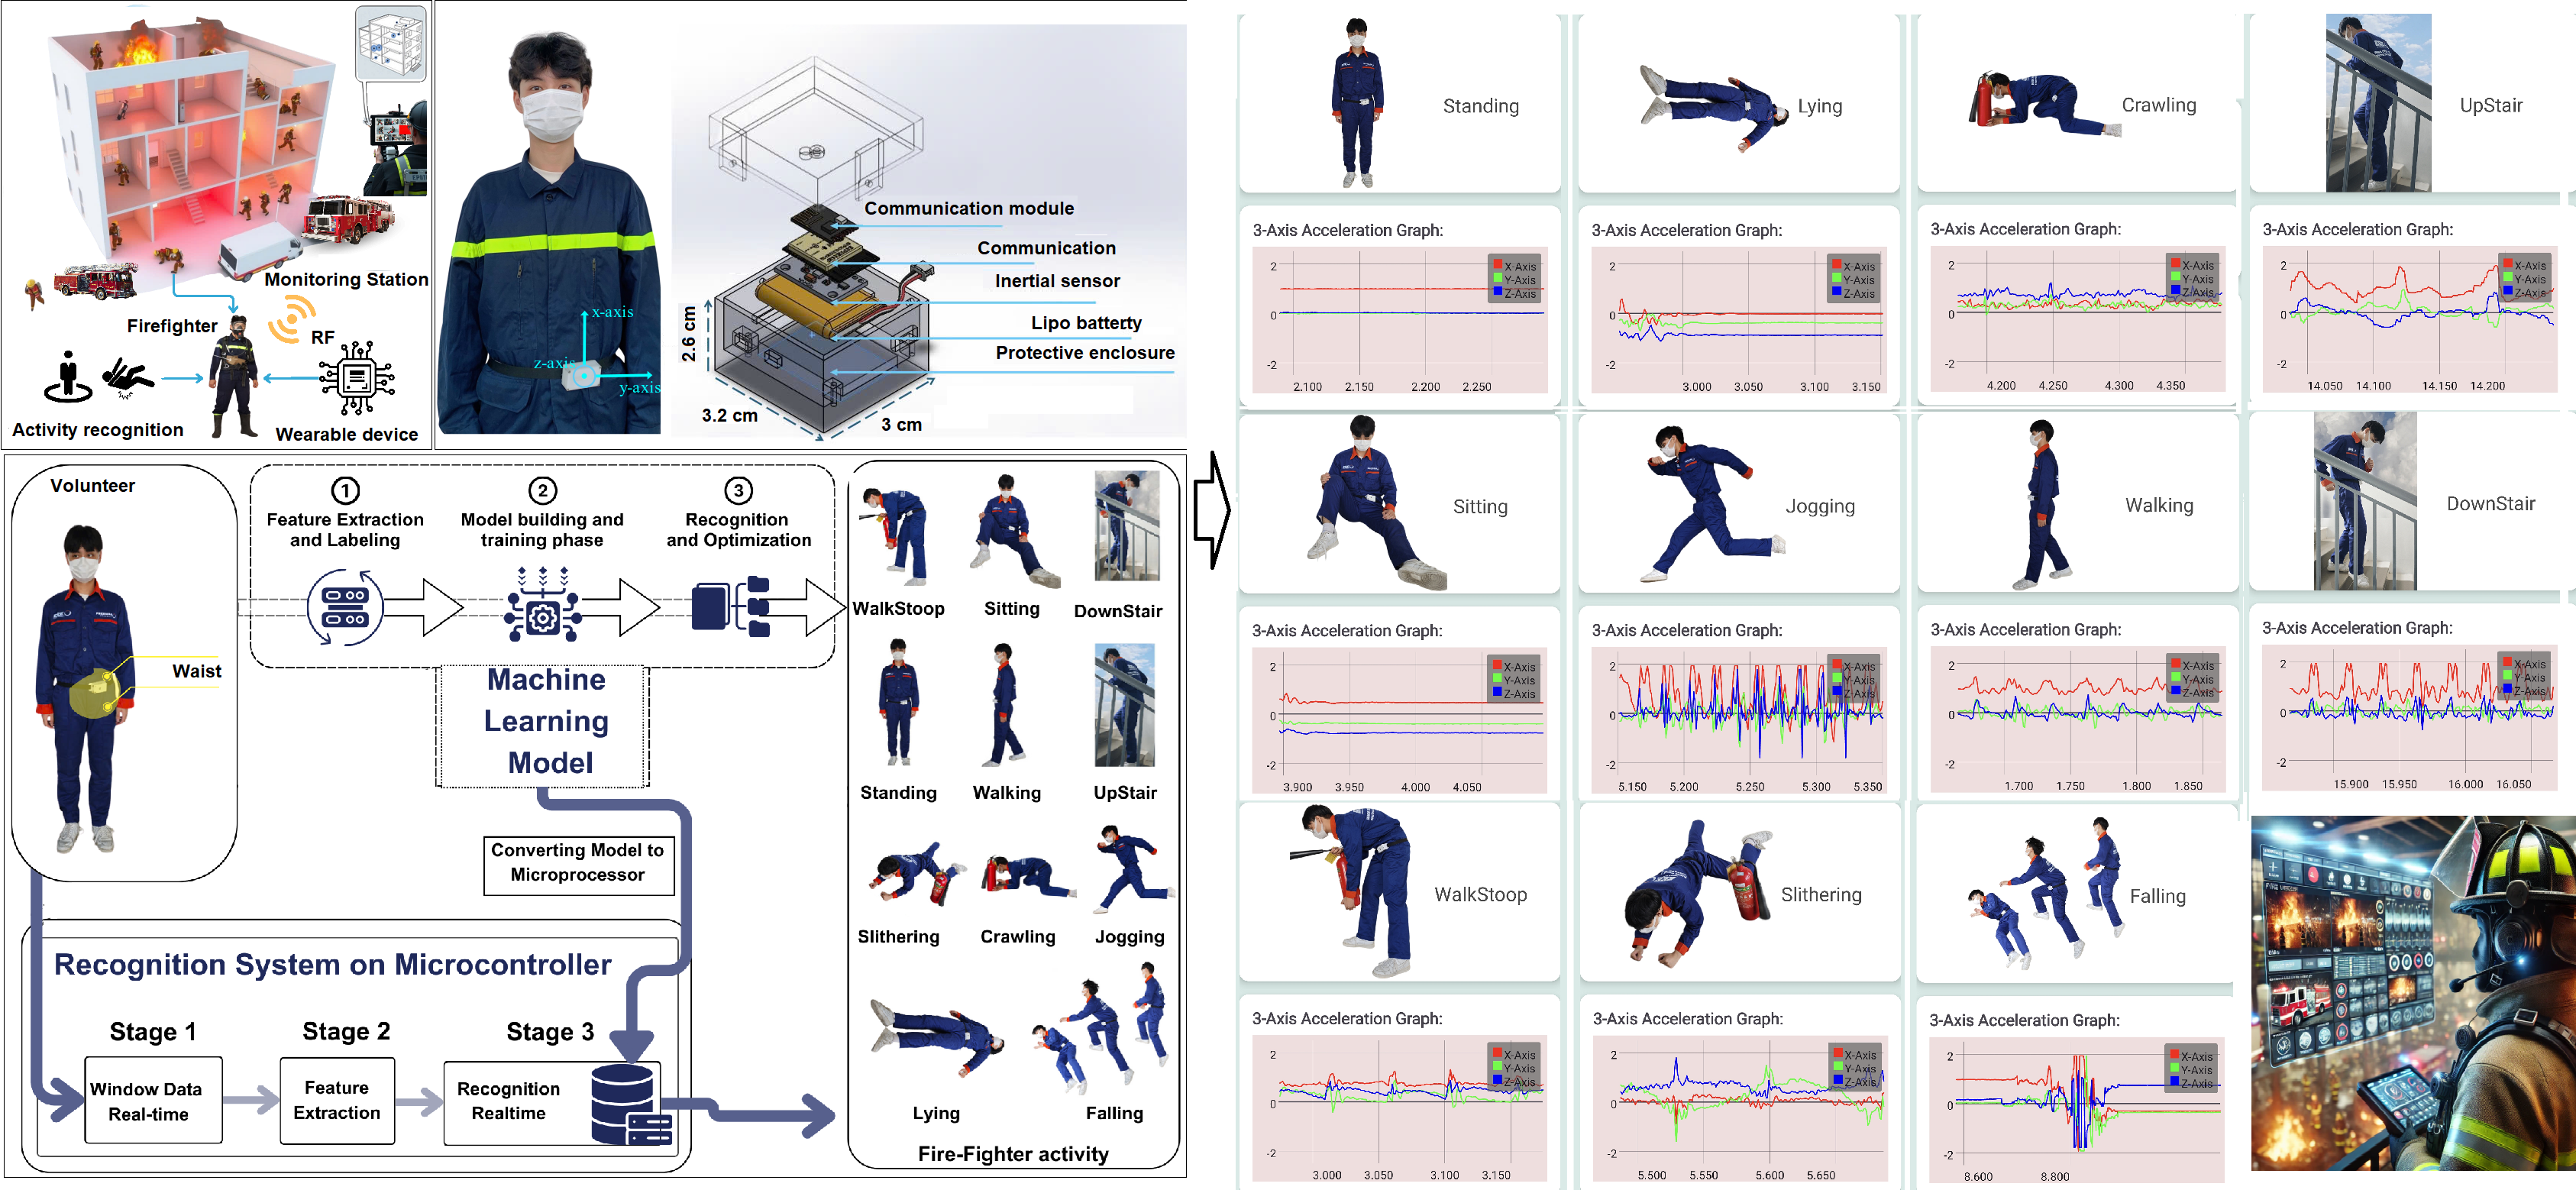
\includegraphics[width=2.0\columnwidth]{figure/FirefighterSystemfull.png}}
\caption{System for recognizing activities of firefighters through a waist-worn device, interacting with the command screen via radio frequency wave.}
\label{Firefighter_System}
\end{figure*}

Fig.~\ref{Firefighter_System} illustrates the overall architecture and operation flow of the proposed FAR system. This system is designed to monitor and assist commanders in tracking the operational status of each team member. Each firefighter is equipped with a compact wearable device mounted at the waist, capable of recognizing and transmitting real-time activity data to a central device controlled by the commander. This central device visually displays the activity status of team members, aiding in timely decision-making during emergency situations.

\begin{table}[h]
\caption{Hardware configuration and experimental platform.}
\label{table_hardware}
\begin{threeparttable}
\renewcommand{\arraystretch}{1.2} % Điều chỉnh khoảng cách giữa các hàng
\resizebox{\columnwidth}{!}{ % Co bảng theo chiều rộng của cột
\begin{tabular}{
    >{\centering\arraybackslash}m{0.12\linewidth}
    >{\arraybackslash}m{0.2\linewidth}
    >{\arraybackslash}m{0.58\linewidth}}
\noalign{\hrule height 1.2pt} % Dòng kẻ tiêu đề đậm hơn
\rowcolor{gray!20}\textbf{Module} & \textbf{Component} & \textbf{Specification} \\
\noalign{\hrule height 1.2pt} % Dòng kẻ tiêu đề đậm hơn
\multirow{5}{*}{\makecell{Wearable\\device}}
& ADXL345 & 3-axis accelerometer \\
& \footnotemark[1]ESP32 & 520~KB RAM, 448~KB ROM, 4~MB flash \\
& Micro SD card & 2~GB \\
& Communication & 433~MHz; 8000~meters; 2.4~Kbps \\
& Battery & Li-ion, 2000~mAh \\
\hline
\multirow{3}{*}{\makecell{Central \\ device}} 
& Communication & 433~MHz; 8000~meters; 2.4~Kbps \\
& ESP32 & 520KB RAM, 448KB ROM, 4~MB flash \\
& Power & Adapter 12~VDC~---2A \\
\hline
\multirow{6}{*}{Server} 
& Chipset & Intel Xeon Silver 4310; 2.1~GHz speed \\
& RAM & 16~GB RDIMM \\
& Hard disk & 2TB IDD NLSAS \\
& Software & Visual studio code\\
& Platform & Windows server 2019\\
& Protocol & Message queuing telemetry transport\\
\noalign{\hrule height 1.2pt} % Dòng kẻ tiêu đề đậm hơn
\end{tabular}
}
\begin{tablenotes}
\footnotesize
\item[1] \url{https://www.espressif.com/}
\end{tablenotes}
\end{threeparttable}
\end{table}

The system is capable of recognizing a wide range of activities including WA, ST, LY, SI, JO, WS, CR, SL, FA, DS and US. The live data corresponding to each activity is plotted in real-time and illustrated in Fig.~\ref{Firefighter_System}. It employs a radio frequency communication module to ensure low-latency data transmission, enabling near-instantaneous updates to the central station. Powered by a 2000~mAh LiPo battery, the device supports extended operations while minimizing the need for frequent recharging. Additionally, a low-power microcontroller processes sensor data and manages communication functions, maintaining high performance with optimized energy efficiency. The system configuration employed in this study is described in Tab.~\ref{table_hardware}.

The system operates in three main stages: real-time data collection through a sliding window, feature extraction, and activity recognition. The extracted features are used to train the ML, which is subsequently optimized and deployed on a microcontroller integrated with the device. This system enables the rapid detection and reporting of critical activities, supporting commanders in monitoring and coordinating team operations in hazardous environments. By enhancing both safety and efficiency, the system is particularly suited for degraded buildings where prior system installation is not feasible and can operate reliably in fire conditions, even during power outages.

\subsection{Dataset}\label{Dataset}

This study utilizes four datasets on human activities, including one private dataset focused on firefighter-specific actions and three public datasets that contain similar human actions.

\subsubsection{Private dataset}

The firefighter activity dataset was collected from a group of 20 male volunteers, all in good health, aged between 22 and 35 years, with heights ranging from 1.6~--~1.8~m and weights from 60~--~80~kg. These volunteers were carefully selected from Phenikaa University and the University of Fire Prevention and Fighting, with no female participants included to ensure uniformity in physical characteristics. Data were collected at a sampling frequency ($F_s$) of 100~Hz and comprised three-axis accelerometer measurements recorded in units of $g$ ($g = 9.8m/s^2$), captured during practical rescue and firefighting drills. Complex activities were sampled more frequently to ensure objectivity in dataset construction. The detailed description and the number of samples for each activity in the private dataset are presented in Tab.~\ref{table_activity_description}. Each activity was performed continuously for at least three minutes, except for the FA activity, which was conducted within 3~--~5~s (seconds). The collected data were stored on a microSD card and recorded at the waist-hip area of the volunteers to ensure accuracy and signal stability. The total data collection time amounted to 371~minutes, with the dataset size exceeding 100~MB. In this study, parameter optimization for the RF model was conducted on a private dataset, while DT, GBDT, SVM, light gradient boosting machine (LBM), and extreme gradient boosting (XGB) models were employed to objectively evaluate the effectiveness of the optimization process.

\begin{table}[h!] % Sử dụng table* để bảng hiện toàn trang
    \caption{Description of firefighter activities on private dataset.}
    \label{table_activity_description}
    \footnotesize
\renewcommand{\arraystretch}{1.2} % Điều chỉnh khoảng cách giữa các hàng
\resizebox{\columnwidth}{!}{ % Co bảng theo chiều rộng của cột
    \begin{tabular}{>{\arraybackslash}m{0.08\linewidth}m{0.77\linewidth}m{0.1\linewidth}}
    \noalign{\hrule height 1.2pt} % Dòng kẻ tiêu đề đậm hơn

      \rowcolor{gray!20}  \textbf{Activity} & \textbf{Description} & \textbf{Samples}\\
        \noalign{\hrule height 1.2pt} % Dòng kẻ tiêu đề đậm hơn
        WA & Moving upright maintaining at least one foot on the ground.&123,932\\
        \hline
        ST & Maintaining an upright posture without movement.&56,016 \\
        \hline
        LY  &Positioning the body on a flat surface with the back touching the ground&82,516 \\
        \hline
        SI & A resting posture with the buttocks and feet in contact with the ground. &63,013\\
        \hline
        JO &A fast movement state with running steps and no more than one foot on the ground at a time.&90,783 \\
        \hline
        WS & Slow walking in a bent or crouched posture. &83,242\\
        \hline
        CR &Moving forward on hands and knees, keeping the torso slightly elevated off the ground.&82,669 \\
        \hline
        SL & Moving close to the ground on hands and knees, with the body parallel to the ground.&90,340\\
        \hline
        FA &Sudden loss of balance resulting in contact with the ground.&129,815 \\
        \hline
        DS  & Descend the stairs on foot at a moderate pace.&151,448\\
        \hline
        US & Climb the stairs on foot at a moderate pace.&157,882 \\
        \noalign{\hrule height 1.2pt} % Dòng kẻ tiêu đề đậm hơn
    \end{tabular}
    }
\end{table}

\subsubsection{Public dataset}
In this study, a new approach is applied, in which falling is considered a behavior rather than merely an isolated event. This perspective differs from previous studies, which often focused separately on either activity recognition or fall detection \cite{Elder_Falling_2019,Firefighter_Falling_2023,Fall_Elder2022}. Therefore, three publicly available datasets, \footnotemark[1]MobiFall\cite {MobiFall2015}, \footnotemark[2]SFDLA \cite{SFDLAdataset2016}, and \footnotemark[3]UniMiB-SHAR \cite{UniMiB_SHAR_2017} containing similar activities, are utilized for comparison to ensure the diversity and objectivity of the study.
\footnotetext[1]{https://www.kaggle.com/datasets/kmknation/mobifall-dataset-v20}
\footnotetext[2]{https://kilyos.ee.bilkent.edu.tr/~billur/}
\footnotetext[3]{http://www.sal.disco.unimib.it/technologies/unimib-shar/}

\subsection{Data processing}
\subsubsection{Segmenting data for non-fall activities}

Assume that an activity signal sequence $\overline{s}[n]$, composed of accelerometer data $\overline{s}[n] = (\overline{a}_x[n], \overline{a}_y[n], \overline{a}_z[n])$, is given, where $\overline{N}$ is the length of the signal sequence $\overline{s}[n]$ and $n \in [1, \overline{N}]$. Here, $\overline{a}_x[n]$, $\overline{a}_y[n]$, and $\overline{a}_z[n]$ represent time-series signals on the respective $x$, $y$, and $z$ axes, obtained from the accelerometer sensor. $\overline{s}[n]$ was recorded by an accelerometer mounted on the firefighter's waist during their activities. 

Sampling frequency plays an important role in HAR system design. For wearable devices targeting elderly users, a low frequency of 1~Hz helps save energy and matches the slower nature of their movements \cite{Thu2022}. In contrast, fast activities require higher frequencies between 50~--~100~Hz to capture more detailed data \cite{ViManhTuyen2024,HongNhung2023,RealtimeOnESP32_2015,wearableFirefirefighter2015}. Selecting an appropriate sampling rate helps balance recognition accuracy, response speed, and hardware constraints. However, processing data at high frequencies requires significant energy and computational resources. In this study, the sampling rate was reduced to 50~Hz to optimize processing efficiency while maintaining the necessary signal quality. To achieve this, a moving average filter was applied, where the average of every two consecutive samples was computed. For each axis $k \in \{x, y, z\}$, the filtered and downsampled signal $s[n]$ is calculated by averaging two consecutive samples from the original signal:
\begin{equation}
\label{resample}
a_k[n] = \frac{\overline{a}_k[2n - 1] + \overline{a}_k[2n]}{2}, \quad n \in [1, N]
\end{equation}
Here, $k$ denotes the $x$, $y$, and $z$ axes, while $s[n]$ is the downsampled signal with size $N = \overline{N}/2$, where $\overline{N}$ is the original signal size. $F_s$ of $s[n]$ is 50~Hz, as applied throughout this study.

To analyze and classify various activities, the continuous signal $s[n]$ was segmented into smaller, equally sized time windows. Window sizes such as 10-second \cite{HongNhung2023}, 8-second \cite{ViManhTuyen2024}, and 6-second \cite{Thu2022}, may cause delays in real-time responses and mix multiple actions within a single window. Previous studies on fall detection for firefighters \cite{Thanhfire2019, Dang2022} and the elderly \cite{HAR_CNN_2025, HAR_DCT_deeplearning2023,DL_Abdi2024} have also employed a 3-second window to achieve a balance between responsiveness and recognition accuracy.

This segmentation was performed by selecting a fixed time duration ($\Delta t=3$~s) for each window and dividing the total duration of the recorded signal into time windows ($W_j[n]$). Each $W_j[n]$ contains $M$~samples of $a_x[n]$, $a_y[n]$, and $a_z[n]$, corresponding to the time interval $[n_i, n_{i+1}]$, where $n_i$ is the start time of the $j^{th}$ window and $n_{i+1}$ is the end time, marking the point where the next window begins. The duration of each time window is given by $\Delta t = n_{i+1} - n_i$. Let the signal be segmented into $N_{\delta t}$ windows. Within each window $W_j[n]$, the accelerometer is represented as: $W_j[n] = (a_x[n], a_y[n], a_z[n]), \quad n \in [n_i,n_{i+1}], \quad j \in [1,N_{\delta t}]$. All segmented activity data were divided into training and testing sets with a 60/40 split.

\subsection{Labelling}

The data labeling process involved segmenting the accelerometer data into windows and assigning labels corresponding to specific firefighter activities. Each activity was performed naturally by the volunteers in simulated scenarios designed to closely reflect practical conditions. The actions were directly observed and manually labeled by two supervisors to ensure annotation accuracy. The steps are as follows:

\textbf{Step 1:} There are 11 activities (WA, ST, LY, SI, JO, WA, CR, SL, FA, DS, US), each corresponding to a unique label from 0 to 10.

\textbf{Step 2:} Sequential segmentation and labeling.

Dataset is processed sequentially for each action. For activity \( k \) (\( k = 0, 1, \dots, 10 \)), the data is segmented into \( N_{\delta t}\) time windows and labeled before moving on to the next activity.

\textbf{Step 3:} Label assignment. 
For each window $W_j[n]$ belonging to activity $k$, the label $L_j$ is assigned as $L_j = k$. Labels are assigned sequentially. After labeling all windows for activity $k$, the process continues with activity $k+1$, where the new label is assigned as $L_j = k+1$. The labeled dataset consists of pairs of windows and their corresponding labels, denoted as $\{(W_1[n], L_1), (W_2[n], L_2), \dots, (W_{N_{\delta t}}[n], L_{N_{\delta t}})\}$. Here, $L_j$ is determined by the activity associated with window $W_j[n]$. Labels are only updated after completing the labeling process for all data of the current activity. This approach ensures that each window $W_j[n]$ is linked to a single activity and assigned a unique label $L_j$.

\subsubsection{New data processing pipeline for falling detection}

\begin{figure*}[h!]
\centering
\footnotesize
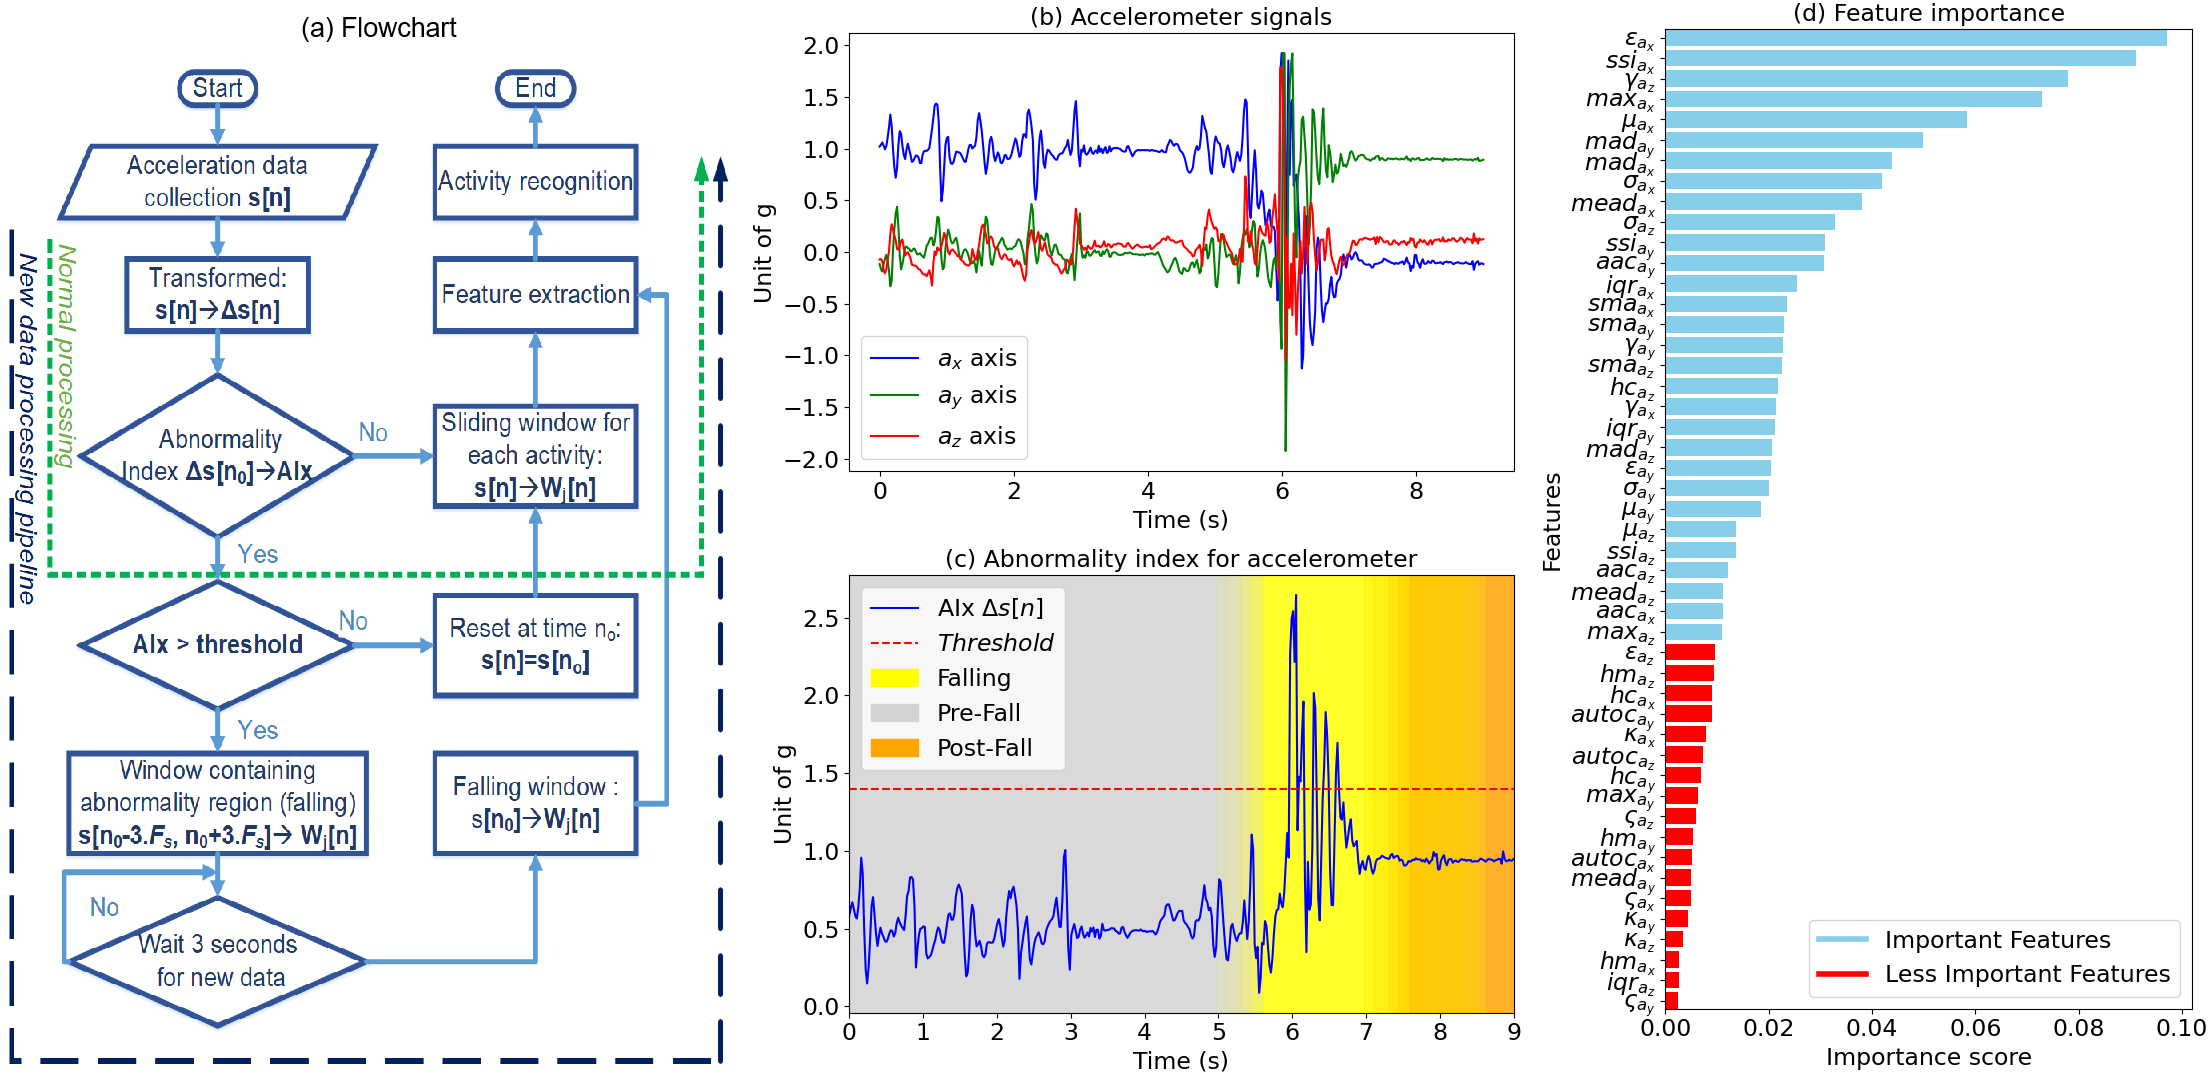
\includegraphics[width=1.0\linewidth]{figure/pipeline.png}
\caption{Flowchart of the abnormality detection and data processing pipeline (a), signal variation during FA activity (b), abnormality detection results (c), and feature importance for activity recognition (d).}\label{pipeline}
\end{figure*}

The above time windows were used only to recognize routine, repetitive activities, while the fall activity was segmented separately, based on detecting abnormal points that exceeded a threshold to create a signal region containing this activity. Fig.~\ref{pipeline}-a illustrates a newly proposed pipeline for abnormality detection in data processing. The notable differences are highlighted in dark blue, representing the new process. In contrast, the green arrows depict the conventional process used previously. This approach enhances the detection of motion and fall actions while improving accuracy. This approach is designed to detect motion and fall actions while improving accuracy. A key highlight of the detection process is the modification of how data windows are generated when a fall event occurs. Specifically, instead of using a fixed sliding window, the system creates a specialized data window that includes the abnormal region (\(s[n_0 - 3 \cdot F_s, n_0 + 3 \cdot F_s]\)) around the detected fall time \(n_0\). This approach focuses on the critical region, and improves the performance of motion recognition and enhances the effectiveness of fall detection compared to conventional data processing methods. The abnormality detection method is carried out through the following steps:

\textbf{Step 1: Detecting the abnormality index.} The abnormality index ($AIx$) represents sudden variations in the accelerometer signal $s[n]$ at a specific moment. In this study, $AIx$ is used to identify the moment when the firefighter falls and makes contact with the ground. To calculate $AIx$, the accelerometer signal $s[n]$ is transformed into a variation sequence $\Delta s[n]$, which quantifies the combined deviations of the three acceleration components $(a_x[n], a_y[n], a_z[n])$ from their respective means over a defined time mini window $\Delta W$. Thanh et al.~\cite{Elder_Falling_2019} indicated that the minimum time for the flight of fall period, from the onset of the fall until the body initially reaches the ground, is approximately 0.34~s. Thus, This study adopts $\Delta W=0.5$~s as the minimum time for detecting $AIx$. The signal transformation process and the detection of areas corresponding to fall-related phases based on the abnormality index are illustrated in Fig.~\ref{pipeline}-b and Fig.~\ref{pipeline}-c.

\begin{equation}\footnotesize
\centering
\begin{aligned}
\Delta s[n] &= \sqrt{\sum_{k \in \{x, y, z axes\}} \left( a_k[n] - \frac{1}{N} \sum_{n=1}^{N} a_k[n] \right)^2}
\end{aligned}
\end{equation}

$AIx$ is detected if $\Delta s[n_0]$ at time $n_0$  exceeds a predefined $threshold$.
\begin{equation}\footnotesize
AIx =
\begin{cases} 
\Delta s[n_0], & \text{if } \Delta s[n_0] > \textit{threshold}=1.8\,g, \\
0, & \text{otherwise}.
\end{cases}\\
\end{equation}
where, $threshold$ is the upper threshold value proposed by Thanh \cite{Thanhfire2019}.

\textbf{Step 2: Collecting data around the abnormal event.} 

After detecting an abnormality at time \( n_0 \) from the accelerometer signal, additional data is collected for 3~s before and after this event $W_j[n]$ with $n \in [n_0-3\cdot F_s,n_0+3\cdot F_s]$.


\textbf{Step 3: Processing the collected data.} 
The data collected during this time window is used to analyze and determine the severity of the fall event. The analysis process may involve extracting features from the accelerometer signals, such as the mean, standard deviation, or characteristic frequency of the signal, for the purpose of detecting falls (Fig.~\ref{pipeline}-c).


\subsection{Feature extraction}

Feature extraction is essential in recognizing activity \cite{ViManhTuyen2024,HongNhung2023,ImportandFeature2023}. In the study by Chai et al. \cite{CHAI_FIRE2024}, FAR was utilized to evaluate the effectiveness of training and physical fitness exercises for firefighters, achieving an accuracy of over 90~\%. They investigated 654 features extracted from surface electromyography, accelerometer, and gyroscope data for firefighting activity recognition (25 time and 6 frequency domain feature types). To optimize computation, only low-complexity time-domain features for accelerometers are considered in this study, following the feature selection approach proposed by Chai et al. However, autoregressive coefficients involve computationally expensive operations, making it unsuitable for microcontroller implementation. Therefore, the selection from 16 time domain feature types is evaluated and optimized, including energy ($\varepsilon$), mean absolute deviation ($mad$), signal magnitude area ($sma$), mean ($\mu$), standard deviation ($\sigma$), simple square integral ($ssi$), average amplitude change ($aac$), maximum ($max$), interquartile range ($iqr$), hjorth mobility ($hm$), median absolute deviation ($mead$), range ($\gamma$), skewness ($\varsigma$), kurtosis ($\kappa$), autocorrelation ($autoc$), hjorth complexity ($hc$).

To reduce the number of features and optimize the performance of the recognition model, features with low importance were removed to decrease model complexity, while maintaining accuracy. A study \cite{ImportandFeature2023} proposed an improved method for RF by gradually eliminating less important features. This approach identifies and removes irrelevant features during model training, leading to improved classification accuracy. Similarly, research \cite{featureSelection2021} suggested using the standard deviation of the information gain values generated by each feature as a threshold. Features with values equal to or above this threshold are retained, while those below are discarded. In Fig.~\ref{pipeline}-d, the standard deviation of importance scores is approximately 0.02, indicating the spread of feature importance values. Therefore, a threshold of 0.01, chosen as half the standard deviation, was applied to eliminate features with minimal importance, effectively reducing the number of features while preserving model performance. As a result, 30 optimal features were selected, and their details are summarized in Tab.~\ref{table_feature}.

\begin{table*}[h!]
\centering
\footnotesize
\caption{Summary of information describing the features used.}
\label{table_feature}
\setlength{\extrarowheight}{2pt}
\renewcommand{\arraystretch}{1.5} % Điều chỉnh khoảng cách giữa các hàng
\resizebox{\textwidth}{!}{ % Co bảng theo chiều rộng của trang
\begin{tabular}{m{0.165\linewidth}m{0.05\linewidth}m{0.45\linewidth}m{0.3\linewidth}}
\noalign{\hrule height 1.2pt} % Dòng kẻ tiêu đề đậm hơn
\rowcolor{gray!20}\textbf{Feature types} & \textbf{Axis} & \textbf{Description} & \textbf{Formula} \\
\noalign{\hrule height 1.2pt} % Dòng kẻ tiêu đề đậm hơn
Energy & x, y & The square root of the average of the squared signal values on x, y axes&
\(\varepsilon_{a_{k}} = \sqrt{\frac{1}{M} \sum_{n=1}^{M} {a_k^{2}[n]}}\)\\

Mean absolute deviation & x, y, z& Mean deviation from the average value on x, y, z  axes.&
\(\text{mad}_{a_{k}} = \frac{1}{M} \sum_{n=1}^{M} \left|a_{k}[n] - \mu_{a_{k}}\right|\)\\

Signal
magnitude area&x, y, z& Sum of absolute magnitude of signal on x, y, z axes.&
\(\text{sma}_{a_k} = \sum_{n=1}^{M} \left|a_k[n]\right|\) \\

Mean& x, y, z& Average value of the signal on x, y, z axes.&
\(\mu_{a_{k}} = \frac{1}{M} \sum_{n=1}^{M} a_{k}[n]\) \\

Standard deviation &x, y, z& Signal dispersion around the mean on x, y, z axes.&
\(\sigma_{a_{k}} = \sqrt{\frac{1}{M} \sum_{n=1}^{M} \left(a_{k}[n] - \mu_{a_{k}}\right)^2}\) \\

Simple square integral& x, y, z& Sum of the squared values of the signal on x, y, z axes.&
\(\text{ssi}_{a_k} = \sum_{n=1}^{M} a_k[n]^2\) \\

Average amplitude change&x, y, z& Mean between consecutive samples on x, y, z axes.&
\(\text{aac}_{a_k} = \frac{1}{M-1} \sum_{n=1}^{M-1} \left| a_k[n+1] - a_k[n] \right|\) \\

Maximum&x, z& Maximum value of the signal on x, z axes.&
\(\text{max}_{a_{k}} = \max(a_{k}[n])\) \\

Median absolute deviation &x, z& Median deviation from the median value on x, z axes.&
\(\text{mead}_{a_k} = \text{median}\left(\left|a_k[n] - \text{median}(a_k)\right|\right)\) \\

Interquartile range&x, y& Difference between the 75th and 25th percentiles on x, y axes.&
\(\text{iqr}_{a_k} = Q_3(a_k[n]) - Q_1(a_k[n])\) \\

Hjorth complexity & z 
& \multicolumn{2}{l}{Measures the mobility of the signal on z axis:
$\displaystyle
\text{hc}_{a_k} = \frac{ \text{hm}_{\Delta a_k} }{ \text{hm}_{a_k} }
\quad with \quad
\text{hm}_{a_k} = \sqrt{
\frac{
\frac{1}{M-1} \sum\limits_{n=1}^{M-1} (a_k[n+1] - a_k[n])^2
}{
\frac{1}{M} \sum\limits_{n=1}^{M} (a_k[n] - \mu_{a_k})^2
}
}
$
} \\


Range & x, y, z& Range between max and min values on x, y, z axes.&
\(\gamma_{a_{k}} = \max(a_{k}[n]) - \min(a_{k}[n])\) \\


\noalign{\hrule height 1.2pt} % Dòng kẻ tiêu đề đậm hơn
\end{tabular}
} % Đóng \resizebox
\end{table*}


\subsection{Optimization of RF parameters on microcontrollers}

Suppose dataset \( \mathcal{D} = \{(feat_j, L_j)\}_{j=1}^{N_{\delta t}} \), where:
\begin{itemize}
    \item \( L_j \in \{1, 2, \dots, 11\} \) is the output label of \( feat_j \), with 11 labels corresponding to different activities.
    
    \item \textbf{RF structure:} the model consists of \( n\_\text{estimators} \) decision trees, denoted as \( T_1, T_2, \dots, T_{n\_\text{estimators}} \), with each tree limited to a maximum depth of \( \text{max\_depth} \). Each DT is built from a different subset of the training data \( \mathcal{D} \) using the bootstrap sampling technique. Each tree \( T_e \) is trained on a subset \( \mathcal{D}_e \subset \mathcal{D} \) and makes predictions for specific inputs.

    \item \textbf{Prediction using RF:} For an input feature vector \( feat_j \in \mathcal{D} \), each tree in the forest makes a prediction:
    \begin{equation*}
        T_e(feat_j) \in \{1, 2, \dots, 11\}, \quad e = 1, 2, \dots, n\_\text{estimators}.
    \end{equation*}
    where \( T_e(feat_j) \) is the predicted label of the \( e \)-th tree.

    \item \textbf{Final prediction:} The final predicted label is determined by majority voting over the predictions of all trees.
    \begin{equation*}
        \hat{L}_j = \text{Voting}(T_1(feat_j), T_2(feat_j), \dots, T_{n\_\text{estimators}}(feat_j)).
    \end{equation*}
\end{itemize}


RF~\cite{DaoHieu2022,ViManhTuyen2024} with optimized weights is a suitable solution due to its compact size and low inference latency. However, RAM on microcontrollers is typically constrained, as it must concurrently support real-time data processing and system-level operations, while flash memory is occupied by firmware, sensor buffers, and configuration data \cite{TinyML2023}. As a result, the available capacity for deploying tinyML is limited \cite{SurveyTinyML2023}, and recent studies \cite{Tiny_machine_on_microcontroller,TinyMLOnEmbedded2025,RIOT_tinyML2025} have typically deployed models on microcontrollers with approximately 1~MB of non-volatile memory.

Alg.~\ref{OptimizationRandomForest} describes the hyperparameter tuning process for the RF model, based on an F1-score micro ($F1_{mi}$) and the constraint that the model size must not exceed 1~MB. To meet the requirement of optimizing the model for deployment on memory-constrained microcontrollers, two key hyperparameters, $n\_\text{estimators}$ and $\text{max\_depth}$, were carefully adjusted. Their values were systematically explored within the range of 1~--~50. For each parameter combination, the model was evaluated using $F1_{mi}$ and as the model size. These parameters have a significant impact on both the model size and recognition accuracy \cite{Tuning_RandomForest2023, Tuning_RandomForest2024}. Selecting the optimal configuration ensured that the model remained compact while maintaining good recognition performance. The same hyperparameter tuning procedure was applied to all machine learning models in Tab.~\ref{table_model_config}, using the same training data and evaluated on the same testing data.


\begin{algorithm}
\footnotesize
\caption{\footnotesize Hyperparameter optimization for ML}
\label{OptimizationRandomForest}
\KwIn{Full dataset $\mathcal{D}$, model size limit = 1~MB}
\KwOut{Optimized parameters $(n\_estimators^*, max\_depth^*)$ and corresponding RF model}

Split $\mathcal{D}$ into $\mathcal{D}_{train}$ (60~\%) and $\mathcal{D}_{test}$ (40~\%) \;
Initialize $best\_score \leftarrow 0$, $best\_param \leftarrow$ None \;

\For{$max\_depth$ in [1,2,..,50]}{
    \For{$n\_estimators$ in [1,2,..,50]}{
        Train RF model $clf$ on $\mathcal{D}_{train}$ with current parameters \;
        Evaluate $clf$ on $\mathcal{D}_{test}$, compute $score_{val}=f1_{mi}$ \;

        \If{$model\_size(clf) < 1$~MB}{
            Perform 5-fold cross-validation on $\mathcal{D}$ to obtain $score_{cv}$ \;
            \If{$|score_{val} - score_{cv}| \leq \varepsilon$ \textbf{and} $score_{val} > best\_score$}{
                $best\_score \leftarrow score_{val}$ \;
                $best\_param \leftarrow (n\_estimators, max\_depth)$ \;
                $best\_model \leftarrow clf$ \;
            }
        }
    }
}

Export $best\_model$\;
\end{algorithm}

The implementation of embedding the RF model into a microcontroller is detailed, ensuring that the hardware's memory and computational limitations are effectively managed.

\begin{itemize}
    \item \textbf{Model conversion and export:}
    \begin{itemize}
        \item Import the model conversion library using: \texttt{from micromlgen import port}.
        \item Convert the trained model ($clf$) into C code: \texttt{model\_code = port($clf$)}.
        \item Save the converted model as a header file:\\
            \texttt{with open("random\_forest.h", "w") as file:}
            \texttt{file.write(model\_code)}
    \end{itemize}

    \item \textbf{Model integration:}
    \begin{itemize}
        \item Embed the header file \texttt{random\_forest.h} into the microcontroller firmware: \\
        \texttt{\#include "random\_forest.h"}.
        \item Initialize the RF model in the microcontroller using: \\\texttt{Eloquent::ml::port::RF rf;}.
    \end{itemize}

    \item \textbf{Deployment and execution:}
    \begin{itemize}
        \item For each input feature vector (\( feat_j \)): 
          $\hat{L}_j=$\texttt{rf.predict($feat_j$);}
    \end{itemize}
\end{itemize}


\section{Experiments and results}
\subsection{Evaluation method}

\begin{itemize}
    \item Accuracy ($acc$) represents the ratio of correct predictions to the total number of predictions.
        
        \begin{equation}
        \footnotesize
        \label{eqACC}
        acc =\frac{TP+TN}{TP+FP+TN+FN}
        \end{equation} 
    \item Sensitivity ($sen$) indicates the model's ability to correctly detect activities that are actually occurring.
        \begin{equation}\label{eqSEN}
        \footnotesize
        sen =\frac{TP}{TP+FN}
        \end{equation} 
    \item Specificity ($spe$) shows the model’s ability to correctly identify activities that are not occurring.
        \begin{equation}\label{eqSPE}
        \footnotesize
        spe =\frac{TN}{TN+FP}
        \end{equation} 
    \item Precision ($pre$) represents the proportion of correctly identified positive activities out of all activities predicted as positive.

        \begin{equation}\label{eqPRE}
        \footnotesize
        pre =\frac{TP}{TP+FP}
        \end{equation}  
\end{itemize}
    
\begin{itemize}
    \item F1-score micro ($F1_{mi}$) is particularly suitable for imbalanced data and F1-score macro ($F1_{ma}$) evaluates the average performance across all activities.

\begin{equation} \label{eqF1score}
\footnotesize
F1  = \frac{2 \times pre\times sen}{pre + sen}
\end{equation}

\begin{equation} \label{eqF1macro}
\footnotesize
F1_{mi}  =  \frac{1}{n} \sum_{i=1}^n \frac{2 \times pre_i \times sen_i}{pre_i + sen_i}
\end{equation}

\begin{equation} \label{eqF1micro}
\footnotesize
F1_{ma}  = \frac{1}{n}\sum_{i=1}^n F1_i
\end{equation}

\end{itemize}

In these equations \ref{eqACC}-\ref{eqF1micro}: $TP$ (true positive) is the number of times the model correctly predicted that an activity was actually occurring; $FP$ (false positive) is the number of times the model incorrectly predicted that an activity was occurring when it was not; $TN$ (true negative) is the number of times the model correctly predicted that an activity was not occurring; $FN$ (false negative) is the number of times the model incorrectly predicted that an activity was not occurring when it actually was; $n$ is the number of activities.

\begin{itemize}
    \item K-fold cross-validation: Dataset $\mathcal{D}$ is partitioned into $k$ folds $\mathcal{D}_1, \mathcal{D}_2, \ldots, \mathcal{D}_k$. $k=5$ is applied in this study.
    
   + For each fold $\mathcal{D}_k$: Train the model with optimized parameter in Tab.~\ref{table_model_config} on the training set $\mathcal{D}_{\text{train}}^{(k)} = \{\mathcal{D} \setminus \mathcal{D}_k\}$.
    
    + Compute the $F1_{mi}^{k}$  for fold $\mathcal{D}_k$.
    
    + Overall performance: $Score_{CV}=\frac{1}{k} \sum_{i=1}^{k}F1_{mi}^{k}$.

\end{itemize}


\subsection{Experimental evaluation}

RFAR was experimentally deployed on volunteers using a wearable device integrated with the proposed model during a drill at the University of Fire Prevention and Fighting in Vietnam.
\subsubsection{Results on private dataset}

\begin{table*}[h!]
\centering
\resizebox{\textwidth}{!}{
\begin{threeparttable}
\caption{Configuration parameters of recognition models on private dataset.}
\label{table_model_config}
\footnotesize
\renewcommand{\arraystretch}{1.2}
\begin{tabular}{
>{\arraybackslash}m{0.05\linewidth}
>{\raggedright\arraybackslash}m{0.25\linewidth}
>{\raggedright\arraybackslash}m{0.06\linewidth}
>{\raggedright\arraybackslash}m{0.06\linewidth}
>{\raggedright\arraybackslash}m{0.06\linewidth}
>{\raggedright\arraybackslash}m{0.06\linewidth}
>{\raggedright\arraybackslash}m{0.06\linewidth}
>{\raggedright\arraybackslash}m{0.06\linewidth}
>{\raggedright\arraybackslash}m{0.06\linewidth}
>{\raggedright\arraybackslash}m{0.06\linewidth}
>{\raggedright\arraybackslash}m{0.06\linewidth}
}
\noalign{\hrule height 1.2pt}
\rowcolor{gray!20}\textbf{Model} & \centering Hyperparameters & $acc$~(\%) & $sen$~(\%) & $spe$~(\%) & $pre$~(\%) & $F1_{mi}$~(\%) & $F1_{ma}$~(\%) & Size~(MB) & Train~(s) & Test~(s) \\
\noalign{\hrule height 1.2pt}

RF &  \textsuperscript{1}$n\_\text{estimators}=17$, \textsuperscript{2}$\text{max\_depth}=14$ & 99.3 &97.0 & 99.6 & 97.1 & 96.1 & 97.0 & 0.921709 & 0.093589 & 0.010951 \\ \hline


XGB& $n\_\text{estimators}=37$, $\text{max\_depth}=14$ & 99.2 & 96.4 & 99.5 & 96.6 & 95.5 & 96.5 & 0.939840 & 0.803459 & 0.047790 \\ \hline

DT &$\text{max\_depth}=16$& 98.5 & 93.3 & 99.1 & 93.6 & 91.7 & 93.5 & 0.056939 & 0.206093 & 0.000996 \\ \hline

GBDT & $n\_\text{estimators}=35$, $\text{max\_depth}=4$ & 98.8 & 94.5 & 99.3 & 94.9 & 93.4 & 94.7 & 0.967428 & 21.020377 & 0.014934 \\ \hline

SVM & \textsuperscript{3}$C\_=29$ & 98.9 & 94.8 & 99.4 & 94.6 & 93.7 & 94.7 & 0.247342 & 21.748170 & 0.091596 \\ \hline

LBM &$n\_\text{estimators}=46$, $\text{max\_depth}=22$ & 99.1 & 96.1 & 99.5 & 96.4 & 95.2 & 96.2 & 0.966480 & 0.226004 & 0.007965 \\
\noalign{\hrule height 1.2pt}
\end{tabular}

\begin{tablenotes}
\footnotesize
\item[1] Number of trees in boosting models.
\item[2] Maximum depth of each DT in the model.
\item[3] Regularization parameter in SVM.
\end{tablenotes}
\end{threeparttable}
}
\end{table*}

\begin{figure*}[h!]
\footnotesize
\centering
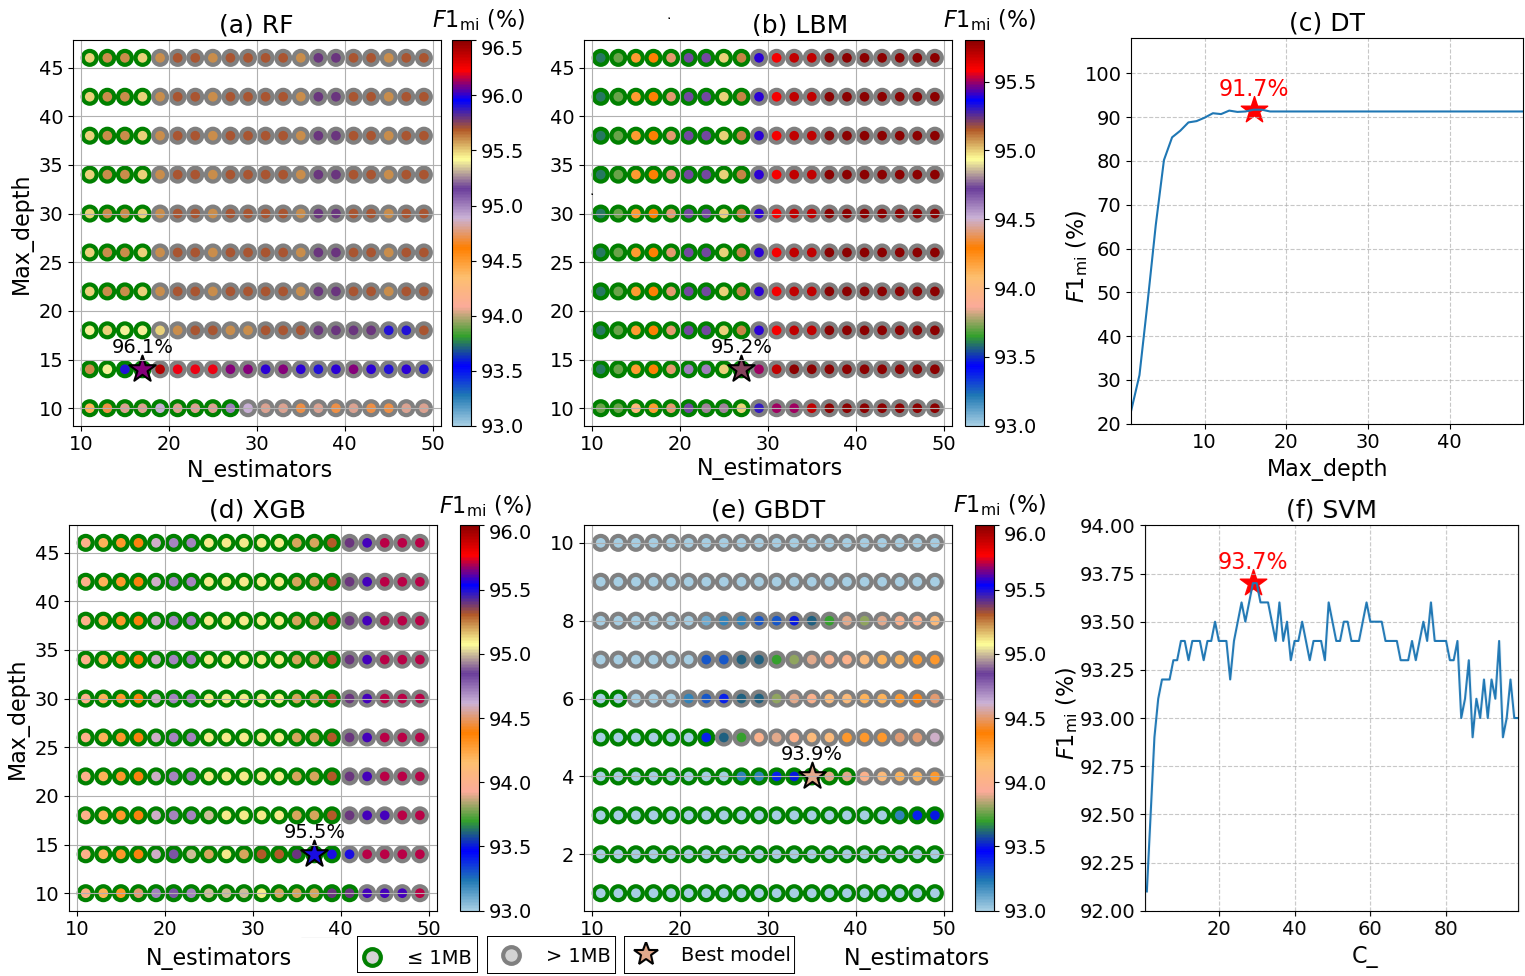
\includegraphics[width=0.9\linewidth, height=8 cm]{figure/find parameter.png}
\caption{$F1_{mi}$ and model size of models (a) RF, (b) LBM, (c) DT, (d) XGB, (e) GBDT, and (f) SVM when tuning parameters.}\label{findparameter}
\end{figure*}

\begin{figure*}[h!]
\centering
\footnotesize
\makebox[\textwidth][c]{ % Bọc thêm dòng này
    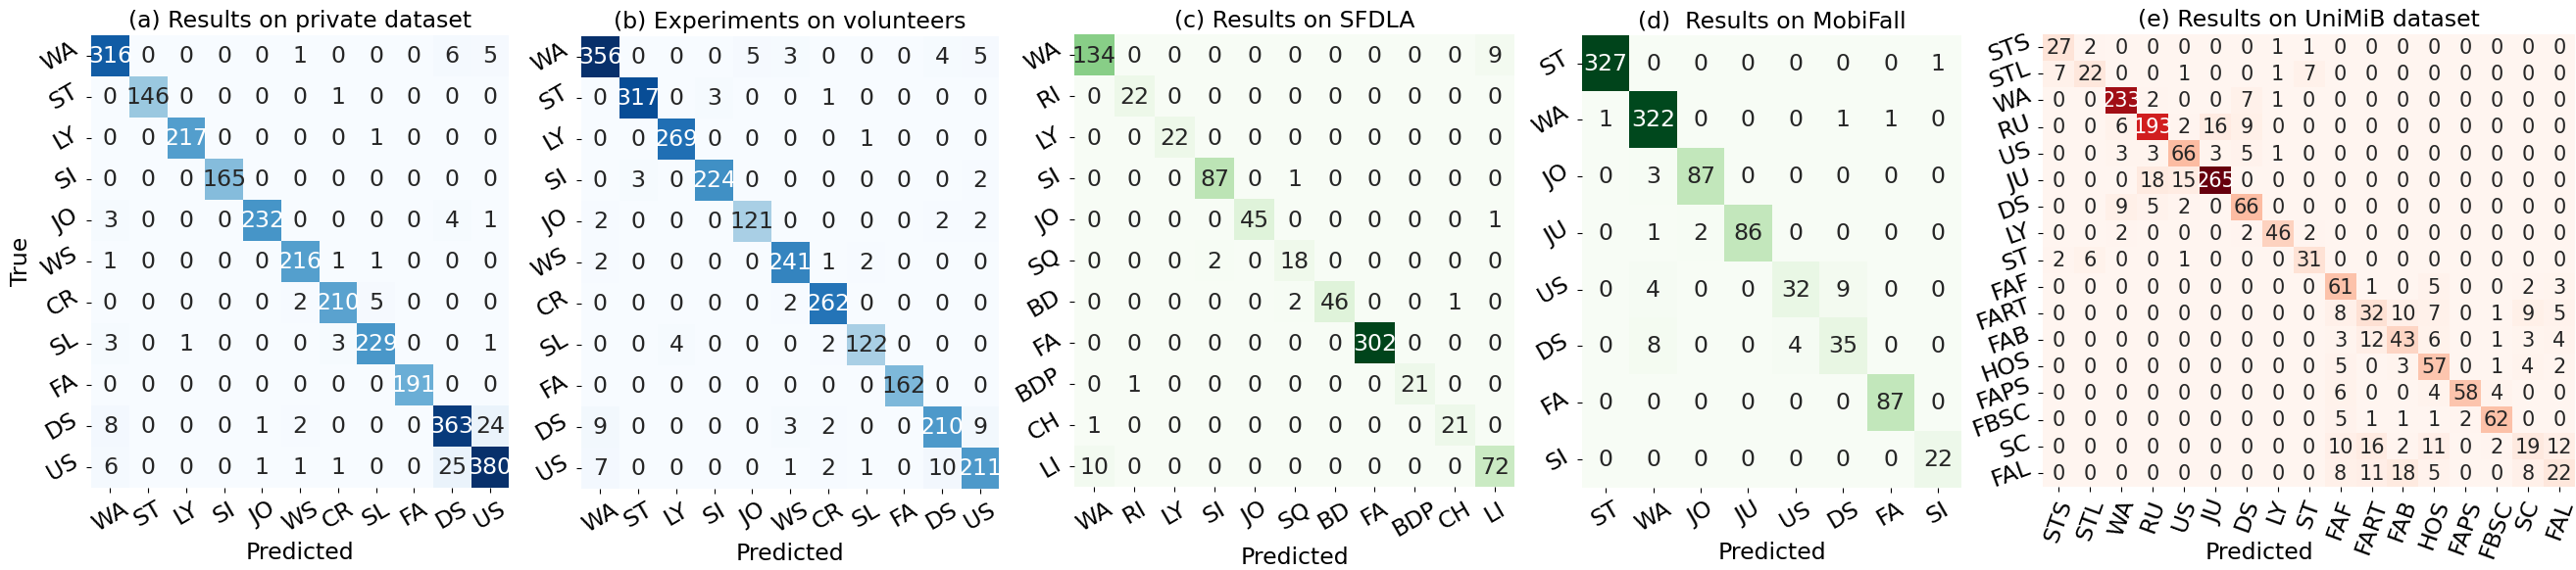
\includegraphics[width=1.05\textwidth]{figure/RFmatrix.png}
}
\caption{The confusion matrix summarizes the results on the (a) private dataset, (b) real-time experiments on volunteers, (c) SFDLA, (d) MobiFall, and (e) UniMiB.} 
\label{RF_matrix}
\end{figure*}

Tab.~\ref{table_model_config} presents the optimal parameter configurations aimed at achieving high $F1_{mi}$ value while ensuring memory size under 1~MB constraints for recognition models. These models were implemented using the scikit-learn library to maintain consistency throughout the training and evaluation processes. As shown in Fig.~\ref{findparameter}, the parameters of each algorithm must be properly constrained to ensure that ML remains under 1~MB in size. XGB (Fig.~\ref{findparameter}-d) is more suitable for a wide configuration range with \text{max\_depth}: 1~--~50 and $n\_\text{estimators}$: 1~--~40, followed by GBDT (Fig.~\ref{findparameter}-e) , which uses $n\_\text{estimators}$: 1~--~50 and \text{max\_depth} below 10. In contrast, RF (Fig.~\ref{findparameter}-a) and LBM (Fig.~\ref{findparameter}-b) adopt more limited parameter ranges to meet the memory constraints. However, RF, XGB, and LBM obtained $F1_{mi}$ over 95~\% with optimal parameters. DT (Fig.~\ref{findparameter}-c) and SVM (Fig.~\ref{findparameter}-f) are more compact, with all configurations under 1~MB, but their $F1_{mi}$ values are lower than those of RF (96.1~\%), XGB (95.5~\%), and LBM (95.2~\%).


Under memory constraints, RF demonstrated a good balance among high accuracy, model size, and processing speed. With a configuration of $n\_\text{estimators}=17$ and $\text{max\_depth}=14$, the model occupied only 0.921709~MB while achieving $acc=99.3~\%$ and over 96~\% across all metrics. In addition, RF provided fast processing with a training time of 0.093589~s on 4171 windows and an inference time of 0.010951~s on 2774 windows, corresponding to approximately 3.95~$\mu$s (microseconds) per prediction. In comparison, models such as XGB ($n\_\text{estimators}=37$, $\text{max\_depth}=14$, 0.939840~MB) and LBM ($n\_\text{estimators}=46$, $\text{max\_depth}=22$, 0.966480~MB) achieved similar accuracy (above 99~\%) but required more trees and longer training times (XGB: 0.803459~s, LBM: 0.226004~s). Although DT achieved the shortest inference time (0.000996~s) with a very small model size (0.056939~MB), its metrics remained above 91~\%.

Fig.~\ref{RF_matrix}-a illustrates the confusion matrix on the private dataset. The RF model correctly recognized most activities, such as WA (316/321), ST (146/148), LY (217/219), SI (165/166), and JO (232/235), reflecting clear separability in their signal patterns. However, notable confusions were observed between similar locomotion activities. Specifically, 24 DS were misclassified as US, and 5 WA as US. These errors likely stem from overlapping motion features during elevation changes or transitions, where acceleration patterns are similar. For instance, DS$\leftrightarrow$US and WS$\leftrightarrow$WA involve actions with comparable gait profiles but differing intensity or direction. CR and SL were generally recognized correctly. However, they showed slightly more confusion with similar low-speed or transitional actions such as WS and LY. This may be caused by signal variation or short data windows. In contrast, static postures like ST and LY were recognized with high accuracy due to low variation within the class. Most misclassifications occurred between activity pairs that share similar movement patterns.


\begin{table}[h!]
    \caption{Activity evaluation metrics from \textnormal{(a)} private dataset and \textnormal{(b)} real-time experiment.}
    \centering
    \label{table_RF_private_realtime}
    \footnotesize
    \renewcommand{\arraystretch}{1.2}
    \resizebox{\columnwidth}{!}{%
    \begin{tabular}{
        >{\centering\arraybackslash}m{0.15\linewidth}
        >{\arraybackslash}m{0.15\linewidth}
        >{\arraybackslash}m{0.12\linewidth}
        >{\arraybackslash}m{0.12\linewidth}
        >{\arraybackslash}m{0.12\linewidth}
        >{\arraybackslash}m{0.12\linewidth}
        >{\arraybackslash}m{0.12\linewidth}
    }
    \noalign{\hrule height 1.2pt}
    \multicolumn{1}{c}{\cellcolor{gray!20} Data} & \cellcolor{gray!20} Activity & \cellcolor{gray!20} $acc$~(\%) &\cellcolor{gray!20}  $sen$~(\%) & \cellcolor{gray!20} $spe$~(\%) & \cellcolor{gray!20} $pre$~(\%) &\cellcolor{gray!20} $F1$~(\%) \\\noalign{\hrule height 1.2pt}
    \multirow{12}{*}{\makecell{(a) Private\\dataset}} & WA & 98.8 & 96.3 & 99.1 & 93.8 & 95.0  \\
    & ST & 100 & 99.3 & 100 & 100 & 99.7  \\
    & LY & 99.9 & 99.5 & 100 & 99.5 & 99.5 \\
    & SI & 100 & 100 & 100 & 100 & 100  \\
    & JO & 99.6 & 96.7 & 99.9 & 99.1 & 97.9 \\
    & WS & 99.7 & 98.6 & 99.6 & 97.3 & 98.0 \\
    & CR & 99.5 & 96.8 & 99.8 & 97.2 & 97.0 \\
    & SL & 99.5 & 96.6 & 99.7 & 97.0 & 96.8 \\
    & FA & 100 & 100 & 100 & 100 & 100  \\
    & DS & 97.5 & 91.2 & 98.5 & 91.2 & 91.2  \\
    & US & 97.7 & 91.8 & 98.7 & 92.5 & 92.1  \\ \cline{2-7}
    & Overall & 99.3 & 95.9 & 99.6 & 96.4 & 96.1 \\
    \hline
    \multirow{11}{*}{\makecell{(b) Real-time\\experiment}} & WA & 98.6 & 95.4 & 99.1 & 94.7 & 95.1  \\
    & ST & 99.7 & 98.8 & 99.9 & 99.1 & 98.9  \\
    & LY & 99.8 & 99.6 & 99.8 & 98.5 & 99.1  \\
    & SI & 99.7 & 97.8 & 99.9 & 98.7 & 98.2  \\
    & JO & 99.6 & 95.3 & 99.8 & 96.0 & 95.7  \\
    & WS & 99.5 & 98.0 & 99.6 & 96.4 & 97.2  \\
    & CR & 99.6 & 99.2 & 99.7 & 97.0 & 98.1  \\
    & SL & 99.6 & 95.3 & 99.8 & 96.8 & 96.1  \\
    & FA & 100 & 100 & 100 & 100 & 100  \\
    & DS & 98.5 & 90.1 & 99.3 & 92.9 & 91.5  \\
    & US & 98.5 & 90.9 & 99.2 & 92.1 & 91.5  \\ \cline{2-7}
    & Overall & 99.4 & 96.4 & 99.6 & 96.6 & 96.2 \\

    \noalign{\hrule height 1.2pt}
    \end{tabular}
    }
\end{table}

Tab.~\ref{table_RF_private_realtime} summarizes the performance metrics of the proposed method across eleven activities, evaluated on the private dataset and real-time experiments. On the private dataset (Tab.~\ref{table_RF_private_realtime}-a), activities were recognized with high and stable performance across evaluation metrics, with minor variations among actions. Actions such as ST, SI, and FA reached $100~\%$ in $acc$, $sen$, $spe$, $pre$, and $F1$. Other activities, including LY, SL, JO, CR, and WA, also achieved high values, with most metrics exceeding $95~\%$. In contrast, US and DS showed relatively lower results. Specifically, US achieved $sen=91.8~\%$ and $F1=92.1~\%$, while DS reached $sen=91.3~\%$ and $F1=91.2~\%$. However, their $acc$ and $spe$ remained above $97~\%$.

A detailed comparison of ML models after hyperparameter tuning on the private dataset is presented in Tab.~\ref{table_model_config}. RF achieved high values across all evaluation metrics, with $acc$ reaching 99.3~\%, and $sen$, $spe$, $pre$, $F1_{mi}$, and $F1_{ma}$ all around 97~\%. For $acc$, these models achieved high values above $99~\%$, suggesting that extracted features are highly discriminative across activities. In terms of $sen$, RF recorded the highest values ($97-97.2~\%$), followed by XGB and LBM (around $96.6~\%$). DT and SVM showed slightly lower $sen$ ($95.4 - 95.9~\%$), which may affect the detection of less distinctive activities. Regarding $spe$, these models achieved similarly high levels between $99.4~\%$ and $99.6~\%$, suggesting reliable rejection of negative cases. For $pre$, RF achieved $97.1~\%$, while XGB and LBM maintained competitive results at $96.6~\%$. DT and SVM yielded $pre$ ($95.4-95.5~\%$), indicating a marginally higher false positive rate.

Overall, all models exhibited consistent performance across different evaluation settings, as reflected in their stable results across all evaluation metrics. RF maintained relatively balanced scores, while XGB and LBM also achieved stable and comparable outcomes. Although DT, GBDT, and SVM produced lower values, their results remained steady without notable variations. The consistency across both evaluation schemes indicates that the models generalized well, with no indication of overfitting.

\subsubsection{Results of SFDLA dataset}
For the SFDLA dataset, data collected from female participants were excluded. Moreover, sensor data from positions such as the head, right wrist, right thigh, and chest were removed, as these placements were unsuitable for accurately capturing operational movements. After filtering, signals from the waist-mounted sensor were segmented into 3-second windows.

Fig.~\ref{RF_matrix}-c presents the confusion matrix on the SFDLA dataset. The RF model achieved high accuracy across most activity classes. Actions such as RI, LY, and FA were classified without errors in the current test set. Other activities, including SI (87/88), JO (45/46), SQ (squatting) (18/20), BD (bending) (46/49), BDP (bending-pickup), and 21/22 CH (coughing-sneezing), also showed high recognition rates.

 
 WA and LI, which exhibit similar movement patterns, were occasionally misclassified. Specifically, 9 WA were predicted as LI, and 10 LI were predicted as WA. This bidirectional confusion suggests that the two actions share similar motion characteristics, particularly in gait-related patterns. Their differences may be limited in short observation windows or under certain execution styles. A small number of misclassifications occurred in other classes. For instance, one BD instance was predicted as CH. This may be due to a brief forward-leaning posture that appears in both actions during certain time windows.
 
 The overall performance of the proposed RF model on the SFDLA dataset is reported in Tab.~\ref{table:evaluation_public}, with $acc=99.4~\%$, $sen=95.7~\%$, $spe=99.6~\%$, $pre=95.9~\%$, and $F1_{mi}=96.6~\%$. These results indicate that most activities were correctly detected, false positives were limited, and the balance between sensitivity and precision was maintained across classes.


\begin{table}[h!]
    \caption{Comparison of the performance of RF on public datasets.}
    \label{table:evaluation_public}
    \footnotesize
    \renewcommand{\arraystretch}{1.2} % Điều chỉnh khoảng cách giữa các hàng
    \resizebox{\columnwidth}{!}{ 
    \begin{tabular}{>{\arraybackslash}m{0.12\linewidth}
                    >{\arraybackslash}m{0.18\linewidth}
                    >{\arraybackslash}m{0.12\linewidth}
                    >{\arraybackslash}m{0.12\linewidth}
                    >{\arraybackslash}m{0.12\linewidth}
                    >{\arraybackslash}m{0.12\linewidth}
                    >{\arraybackslash}m{0.12\linewidth}} % Cột mới cho bảng 2
        \noalign{\hrule height 1.2pt}
        \rowcolor{gray!20}
        Dataset &
        Size~(MB) &
        $acc$~(\%)&  
        $sen$~(\%)  &   
        $spe$~(\%) & 
        $pre$~(\%) &   
        $F1_{mi}$~(\%) \\
        \noalign{\hrule height 1.2pt}
        SFDLA & 0.750984 & 99.4 & 95.7 & 99.6 & 95.9 & 96.6 \\
        MobiFall & 0.429473 & 99.2 & 92.2 & 99.5 & 94.2 & 96.6 \\
        UniMiB & 0.975449 & 97.4 & 72.6 & 98.6 & 72.2 & 78.2 \\
       \noalign{\hrule height 1.2pt}
    \end{tabular}
    }
\end{table}

\subsubsection{Results of MobiFall dataset}

 The MobiFall dataset includes four types of falls: Forward-lying (FOL), Front-knees-lying (FKL), Back-sitting-chair (BSC), and Sideward-lying (SDL); as well as nine daily activities: ST, WA, JO, Jumping (JU), US, DS, SI, Car-step in (CSI), and Car-step out (CSO). This study focuses on male subjects performing rescue operations inside a burning building. Therefore, certain activities such as BSC, CSI and CSO, are excluded from the analysis. Activities recorded from female volunteers are also not considered. 
 
Recognition performance on the MobiFall dataset is illustrated in Fig.~\ref{RF_matrix}-d, with detailed evaluation metrics summarized in Tab.~\ref{table:evaluation_public}. RF recognized most actions with high accuracy, such as ST (327/328), WA (322/325), JO (87/90), JU (86/89), SI (22/22), and FA (87/87). This result is consistent with the observation from the SFDLA dataset, where ST and WA actions also showed high correctness.

However, the recognition rate decreased for activities with similar posture, such as US (32/45) and DS (35/47). These actions involve stair movement, which shares similar lower-limb motion with WA and JU. The confusion may result from overlapping acceleration patterns during climbing and descending. Misclassifications between US and DS also occurred, indicating that elevation-related activities remain difficult to distinguish using only inertial data.

Most activities were correctly detected, and false detections were limited, despite challenges in distinguishing stair-related actions. RF achieved $acc=99.2~\%$, $sen=92.2~\%$, $spe=99.5~\%$, $pre=94.2~\%$, and $F1_{mi}=96.6~\%$. In summary, the proposed model with optimized parameters reached a good balance on the MobiFall dataset.


\subsubsection{Results of UniMiB dataset}

For the UniMi dataset, 17 activities (AF17) were considered, including StandingUpFS (STS), StandingUpFL (STL), WA, Running (RU), US, JU, DS, LyingDownFS (LY), SittingDown (SI), FallingForw (FAF), FallingRight (FAR), FallingBack (FAB), HittingObstacle (HOS), FallingWithPS (FAPS), FallingBackSC (FASC), Syncope (SC), and FallingLeft (FAL). A major challenge of this dataset is that the smartphone was placed in the front pocket, and its orientation varied significantly between data collection sessions, including cases where the device was inverted or rotated, which made HAR more difficult. Therefore, the actions were preprocessed and mapped to a common orientation when similar activities began.

These activities were categorized into two main groups: (1) normal activities of daily living (ADLs), which included STS, STL, WA, RU, US, JU, DS, LY, and ST; and (2) fall-related activities. The recognition results on the UniMiB dataset are presented in Fig.~\ref{RF_matrix}-e, and the corresponding evaluation metrics are provided in Tab.~\ref{table:evaluation_public}. Some activities reached high recognition accuracy, such as WA with 233/242 (96.3~\%), LY with 46/52 (88.5~\%), and RU with 193/229 (84.2~\%). In addition, transitional activities such as STS (27/31, 87.1~\%), US (66/80, 82.5~\%), and DS (66/82, 80.5~\%) were also well recognized. STL was the most difficult to classify, only reaching 22/38 (57.9~\%). Most STL samples were misclassified as STS or ST, which have similar starting or ending postures.

In contrast, the fall-related activities group, consisting of 8 classes with a total of 879 windows, showed low recognition performance, with only 431 windows correctly recognized. Fall activities were mostly confused with each other. Some actions, such as FAF (61/72, 84.7~\%), FAPS (58/72, 80.6~\%), and FBSC (62/78, 79.5~\%), had relatively good recognition accuracy. However, other activities, such as FART (32/79, 40.5~\%), FAL (22/76, 28.9~\%), and especially SC (19/85, 22.4~\%), showed low recognition accuracy. These falls produced similar acceleration changes at the moment of impact, which reduced the model’s ability to separate them.

With $sen$ and $pre$ only at 71~--~72~\% and $F1_{mi}$ averaging 78.2~\%, the model still had difficulty in recognizing different types of falls (Tab.~\ref{table:evaluation_public}). Compared to the SFDLA and MobiFall datasets, where the model achieved high recognition rates across most activities, UniMiB posed more challenges due to the high number of fall classes and the similarity between them. However, the proposed model was able to accurately distinguish between ADLs and fall-related activities, without misclassifying falls as ADLs. This matches the proposed model's ability to correctly recognize dangerous states such as falls.

\subsection{On device deployment and practical evaluation}
\subsubsection{Volunteer evaluation setup}

\begin{figure}[h!]
\centering
\footnotesize
\includegraphics[width=1\linewidth, height=2.5cm]{figure/demo realtime.png}
\caption{The experimental process on firefighters during rescue and emergency drills.} 
\label{Demorealtime}
\end{figure}


During the drill, the volunteers performed eleven activities under various conditions and repeated each activity multiple times (Fig.~\ref{Demorealtime}). The recognition results are presented in Fig.~\ref{RF_matrix}-b, along with the evaluation metrics summarized in Tab.~\ref{table_RF_private_realtime}-b. In addition, a demo video is provided in the \textbf{Appendix} to illustrate the proposed model’s real-time recognition capability after deployment on a microcontroller. Some actions may exhibit slight display delays due to signal transmission and reception errors.

\subsubsection{Inference time, latency, and computational complexity}

In this study, the step size (sliding window step) equals the interval between two consecutive observations, which determines the time between recognition instances. Under normal conditions, the step size is set equal to the window size (3 s), so recognition is performed every 3 s to minimize energy consumption. When the AIx value exceeds a predefined threshold, the step size is reduced to 0.5 s to increase the recognition frequency, while the window size remains constant at 3 s.

\begin{figure}[h!]
\centering
\footnotesize
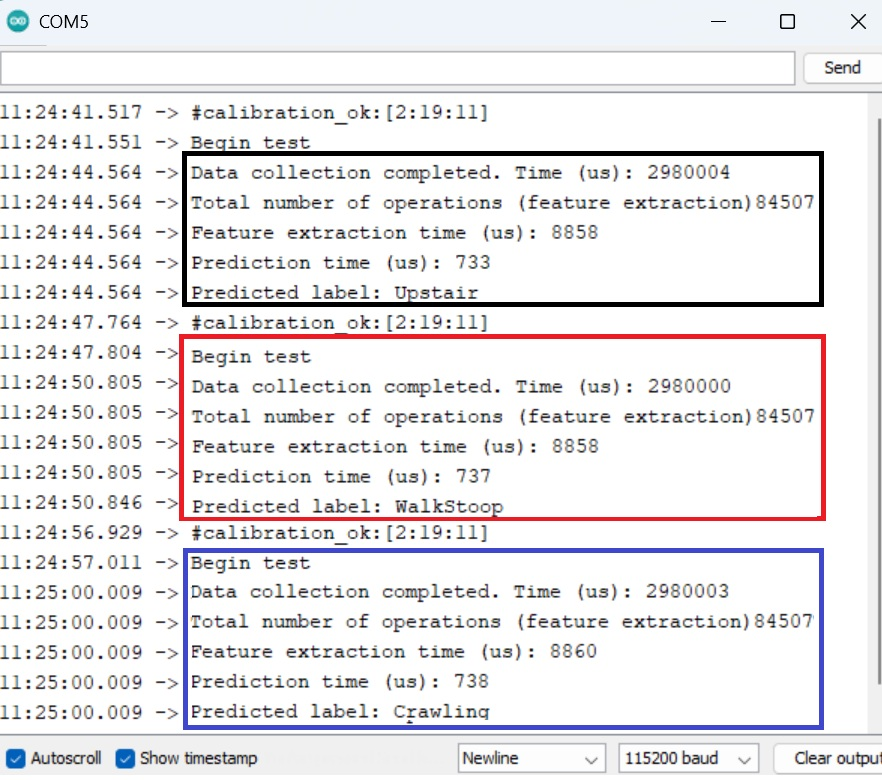
\includegraphics[width=1\linewidth, height=7cm]{figure/Suyluan.png}
\caption{Deployment results of prediction on the microcontroller.} 
\label{suyluan}
\end{figure}

Fig.~\ref{suyluan} shows the actual and computation times on the microcontroller for each processing stage, including data collection, feature extraction, and recognition. With the wearable device integrating an ESP32 microcontroller and an ADXL345 accelerometer, the end-to-end processing flow was evaluated to ensure real-time capability. During operation, the accelerometer samples three-axis data at 50~Hz, and the system collects 450 samples within a 3-second window. Once data collection is complete, feature extraction is performed with approximately 84,507 lines, requiring about 8,858~$\mu$s. The proposed model, with 140,838 instruction lines, completes inference in approximately 733~--~738~$\mu$s. Following recognition, the recognition result is transmitted via SPI at 10~MHz, which takes only about 1.6~$\mu$s and is negligible. 

The proposed model used in this pipeline is implemented directly on performance-constrained microcontrollers. It is configured as a RF with 17 decision trees, each having a maximum depth of 14, and has a compiled size of approximately 0.92~MB. This model has a recognition latency of approximately 9.561--9.596~ms on the ESP32 microcontroller, which is better than that reported in some related studies~\cite{ViManhTuyen2024, Tiny_machine_on_microcontroller,TinyML2023,DeepLearning_latency2020,RIOT_tinyML2025} on TinyML applications for microcontrollers.

\subsubsection{Real-time recognition results}
The real-time recognition performance for actions during the drill is presented in Tab.~\ref{table_RF_private_realtime} and Fig.~\ref{RF_matrix}-b. The model achieved $acc=99.4~\%$, $sen=96.4~\%$, $spe=99.6~\%$, $pre=96.6~\%$, and $F1=96.2~\%$. The FA action was correctly recognized in all 162 windows, with $100~\%$ for all evaluation metrics. Actions such as ST (317/320), LY (269/270), SI (224/229), WS (241/246), JO (121/127), CR (262/264), and SL (122/128) were also recognized with high accuracy. All corresponding metrics exceeded 95~\%. In contrast, WA had 17 misclassifications, mostly as JO, WS, DS, or US. DS and US also had 23 and 21 incorrect predictions, respectively. Similarly, 23/233 DS and 21/232 US were also misclassified. In particular, DS and US recorded $sen$, $pre$, and $F1$ just above 90~\%. The performance degradation for WA, DS, and US is likely due to the similar postures of these activities, which pose challenges for accurate real-time classification with short window sizes. Nevertheless, the number of misclassifications was relatively small and considered acceptable. The real-time results were comparable to those on the private dataset and MobiFall, with all main metrics above 96~\%. Posture transitions and static actions were consistently recognized, as also observed in SFDLA and MobiFall. In contrast, UniMiB included more fall types with similar motion patterns, which made recognition more difficult than in the real-time setting.

In general, the embedded model running on the microcontroller achieved results similar to those of the model tested on the private dataset. Both models showed less than $1~\%$ difference in $acc$, $sen$, $spe$, $pre$, and $F1_{mi}$. Specifically, the model tested on the private dataset reached $acc=99.3~\%$ and $F1_{mi}=96.1~\%$, while the real-time experiment achieved $acc=99.4~\%$ and $F1_{mi}=96.2~\%$. Marginal differences were also observed in $sen$ ($95.9~\%$ and $96.4~\%$) and $pre$ ($96.4~\%$ and $96.6~\%$). These small differences indicate that recognition performance remained stable when the model was applied in practical conditions. This outcome is attributed to the use of an anomaly detection algorithm, which enables the proposed model to more effectively handle posture transitions, thereby reducing noise in practical activity sequences. Additionally, since the volunteers had body shapes similar to those of firefighters, variations in sensor orientation were also minimized.


\section{Discussion}

\subsection{Performance of proposed model}

\begin{table}[h!]
\caption{Comparison of recognition performance on the UniMiB-SHAR dataset.}
\label{tab:Comparison_UniMiB}
\centering
 \footnotesize
\renewcommand{\arraystretch}{1.2} % Điều chỉnh khoảng cách giữa các hàng
\resizebox{\columnwidth}{!}{ % Co bảng theo chiều rộng của cột
\begin{tabular}{>{\arraybackslash}m{0.15\linewidth}%
                >{\arraybackslash}m{0.30\linewidth}%
                >{\arraybackslash}m{0.225\linewidth}%
                >{\arraybackslash}m{0.225\linewidth}}
\noalign{\hrule height 1.2pt}
\rowcolor{gray!20} Dataset & Study & $Acc$~(\%) & $F1_{mi}$~(\%) \\
\noalign{\hrule height 1.2pt}
\multirow{3}{*}{(a) AF17} 
& Proposed & 97.4 & 78.2 \\
& Xu et al.~\cite{HAR_DCT_deeplearning2023} & 97.6 & 79.7 \\
& Teng et al.~\cite{HAR_CNN_2025} & 97.2 & 78.6 \\ \hline
\multirow{4}{*}{(b) AF2} 
& Proposed & 100 & 100 \\
& Al-qaness el al.~\cite{UniMiFall2024} & 99.95 & -- \\
& Kanjilal el al.~\cite{HAR_deeplearning2021} & 99.82 & 98.86 \\
& Iloga at al.~\cite{HMM_UniMiB2021} & 98.85 & -- \\
\noalign{\hrule height 1.2pt}
\end{tabular}
}
\end{table}

Tab.~\ref{tab:Comparison_UniMiB} compares the proposed method with previous studies on the UniMiB-SHAR dataset, based on two activity groups: (a) AF17 and (b) AF2. For AF17, the proposed model achieved $acc=97.4~\%$ and $F1_{mi}=78.2~\%$, which are lower than those of CNN-DCT \cite{HAR_DCT_deeplearning2023} ($acc=97.6~\%$, $F1_{mi}=79.7~\%$) but higher than those of CNN-TSFDU-LW~\cite{HAR_CNN_2025} ($acc=97.2~\%$, $F1_{mi}=78.6~\%$). CNN-DCT is capable of learning frequency-domain features, whereas CNN-TSFDU-LW employs the Temporal-Spatial Feature Decoupling Unit (TSFDU) to separate essential features in order to reduce computational complexity. Both approaches demonstrate strengths in capturing signal characteristics of each activity. However, the accuracy differences between the proposed model and these two models are relatively small. This outcome was achieved due to careful preprocessing, which normalized the input signals from the smartphone into a unified reference frame. For example, signals corresponding to activities such as STS, RU, WA, and FA were aligned to a common direction representing the upright standing posture.

The proposed model demonstrated good and stable recognition performance on the private dataset, with both $acc$ and $F1_{mi}$ exceeding 96~\%. For public datasets, MobiFall and SFDLA achieved comparable results ($F1_{mi}=96.6~\%$). However, UniMiB performed significantly lower, with $F1_{mi}=78.2~\%$. This is mainly due to data collection with varying phone orientations in UniMiB, which increases the challenge for recognition. In addition, the proposed algorithm is well-suited for recognizing firefighter-specific actions, which require frequent posture changes and may involve falls. However, distinguishing specific types of falls remains limited. Furthermore, the device stability considerably affects recognition performance.


\begin{table}[h!]
\centering
\caption{Comparison of the proposed fall detection model with previous other model for firefighter.}
\label{tab:fall_detection_model}
\footnotesize
\renewcommand{\arraystretch}{1.2} % Điều chỉnh khoảng cách giữa các hàng
\resizebox{\columnwidth}{!}{ % Co bảng theo chiều rộng của cột
\begin{tabular}{                >{\arraybackslash}m{0.22\linewidth}%
                >{\arraybackslash}m{0.17\linewidth}%
                >{\arraybackslash}m{0.17\linewidth}%
                >{\arraybackslash}m{0.17\linewidth}
                >{\arraybackslash}m{0.17\linewidth}}
\noalign{\hrule height 1.2pt} % Dòng kẻ tiêu đề đậm hơn
\rowcolor{gray!20}Study & \textbf{$sen$~(\%)}   & \textbf{$spe$~(\%)}  & \textbf{$acc$~(\%)} & \textbf{$GM$~(\%)} \\ \noalign{\hrule height 1.2pt} % Dòng kẻ tiêu đề đậm hơn
 Proposed & 100 & 100 & 100 & 100 \\
 Dang et al.~\cite{Dang2022} & 100 & 98.88 & 99.49 & 99.40 \\
 Chai et al.~\cite{Chai2021} & 92.25 & 94.59 & 94.10 & 93.40 \\
 Thanh et al.~\cite{Thanhfire2019} & 95.89 & 100 & 97.96 & 95.24 \\
\noalign{\hrule height 1.2pt} % Dòng kẻ tiêu đề đậm hơn
\end{tabular}
}
\end{table}

If fall is distinguished from routine daily activities as non-fall instances, the method achieves 100~\% in $sen$, $spe$, $acc$, and $GM$ ($GM = \sqrt{{spe} \times sen}$). Tab.~\ref{tab:fall_detection_model} presents a comparison of the proposed fall detection method with previous studies. Compared to previous studies, the method shows clear improvements. For example, Thanh et al.~\cite{Thanhfire2019} reported $sen$ of 95.89~\%, $spe$ of 100~\%, $acc$ of 97.96~\%, and $GM$ of 95.24~\%. Also, results from Dang et al.~\cite{Dang2022} showed $sen$ of 95.89~\%, $spe$ of 100~\%, $GM$ of 99.4~\%  and $acc$ of 99.49~\%, while the proposed model demonstrates superiority by achieving a better balance between correctly detecting falls and minimizing false positives. The methods proposed by Thanh and Dang share a common limitation in that they rely on fixed signal thresholds, which require manual tuning and are less adaptable to individuals with varying body shapes. Meanwhile, Chai et al.\cite{Chai2021} obtained lower performance with $sen$ of 92.25\%, $spe$ of 94.59~\%, $acc$ of 94.1~\%, and $GM$ of 93.4~\%. The main cause is primarily attributed to the sensor placement on the chest, which increases the likelihood of misclassifying FA and WS. This limitation is effectively addressed in our study through an anomaly detection mechanism that reduces false fall signals during postural transitions or activity changes by the participants.



\begin{table}[h!]
\centering
\caption{Comparison of the proposed fall detection model with previous studies on \textnormal{(a)} SFDLA and \textnormal{(b)} MobiFall datasets.}
\label{tab_Comparison_Fall_SFDLA_MobiFall}
\footnotesize
\resizebox{\columnwidth}{!}{ % Co bảng theo chiều rộng của cột
\renewcommand{\arraystretch}{1.2}
\begin{tabular}{>{\arraybackslash}m{0.14\linewidth}%
                >{\arraybackslash}m{0.28\linewidth}%
                >{\arraybackslash}m{0.12\linewidth}%
                >{\arraybackslash}m{0.12\linewidth}%
                >{\arraybackslash}m{0.12\linewidth}%
                >{\arraybackslash}m{0.12\linewidth}}
\noalign{\hrule height 1.2pt}
\rowcolor{gray!20} Dataset & Study & $sen$~(\%) & $spe$~(\%) & $acc$~(\%) & $GM$~(\%)\\
\noalign{\hrule height 1.2pt}
\multirow{4}{*}{(a) SFDLA} 
& Proposed & 100 & 100 & 100 & 100 \\
& Dang et al.~\cite{Dang2022} & 95.89 & 100 & 97.96 & 97.92 \\
& Thanh et al.~\cite{Thanhfire2019} & 93.33 & 91.67 & 92.50 & 92.50 \\
& Enol et al.~\cite{SFDLA_CNN_LSTM_fall2022} & 100 & 99.97 & 99.97 & 99.98 \\
\noalign{\hrule height 0.8pt}
\multirow{6}{*}{(b) MobiFall} 
& Proposed & 100 & 100 & 100 & 100 \\
& Yi et al.~\cite{MobiFall_Yi_2024} & 100 & 100 & 100 & 100 \\
& Zhang et al.~\cite{MobiFall2024} & 100 & -- & 99.65 & -- \\
& Dang et al.~\cite{Dang2022} & 100 & 98.88 & 99.49 & 99.44 \\
& Hussain et al.~\cite{MobiFall2019} & 96.72 & -- & 98.60 & -- \\
\noalign{\hrule height 1.2pt}
\end{tabular}
}
\end{table}


Table~\ref{tab_Comparison_Fall_SFDLA_MobiFall} presents a comparative evaluation of the proposed fall detection model with existing approaches on the SFDLA and MobiFall datasets. The proposed method achieves consistently high recognition results on the MobiFall, SFDLA, and UniMiB datasets. On the MobiFall dataset, the proposed model achieves $sen$, $spe$, $acc$, and $GM$ all at 100~\%, surpassing previous studies such as Zhang et al.~\cite{MobiFall2024}, which also achieved 100~\% in $sen$. Compared to studies like Thanh \cite{Thanhfire2019}, the proposed model shows significant improvements in $sen$ (100~\%, 90.16~\%, and 100~\%) and $acc$ (100~\%, 96.16~\%, and 99.49~\%). Although both the proposed model and Yi's model achieve an $acc$ of 100~\%, Yi's model relies on 36 features and a complex LSTM architecture, which consumes significantly more resources. Therefore, the proposed approach offers a simpler and more efficient solution for practical applications.

On the SFDLA dataset, the proposed model also maintains maximum performance with all metrics reaching 100~\%, outperforming prior studies such as Dang et al.~\cite{Dang2022} with an $acc$ of 97.96~\% and $GM$ of 97.92~\%, Thanh \cite{Thanhfire2019} with $sen$ of only 93.33~\%. The difference in the results between these two public datasets is attributed to the placement of the data collection device. In the MobiFall dataset, the device used for data collection was a smartphone placed in a pocket near the waist, while in the SFDLA dataset, the device is securely fixed at the waist. This can lead to the SFDLA data being more reliable and less prone to noise compared to the MobiFall dataset.

For AF2 (Tab.~\ref{tab:Comparison_UniMiB}-b), the proposed method achieved 100~\% recognition accuracy for hazardous fall, consistent with results on other datasets as SFDLA and MobiFall. In general, models such as CNN-PCNN \cite{UniMiFall2024}, 1D-CNN \cite{HAR_deeplearning2021}, and HMMs \cite{HMM_UniMiB2021} also achieved very high accuracy for fall actions (over 98~\%). However, the proposed model maintained reliable accuracy while avoiding misclassification between fall actions and ADLs. These models have demonstrated strong capabilities in fall detection and activity recognition, particularly in their ability to automatically extract discriminative features from raw sensor data. However, the proposed model incorporates a processing flow that improves fall detection accuracy by mitigating misclassification caused by transitional or ambiguous movements that resemble falls during daily activity recognition.

\subsection{Sliding window and sampling frequency}

\begin{figure*}[h!]
\footnotesize
\centering
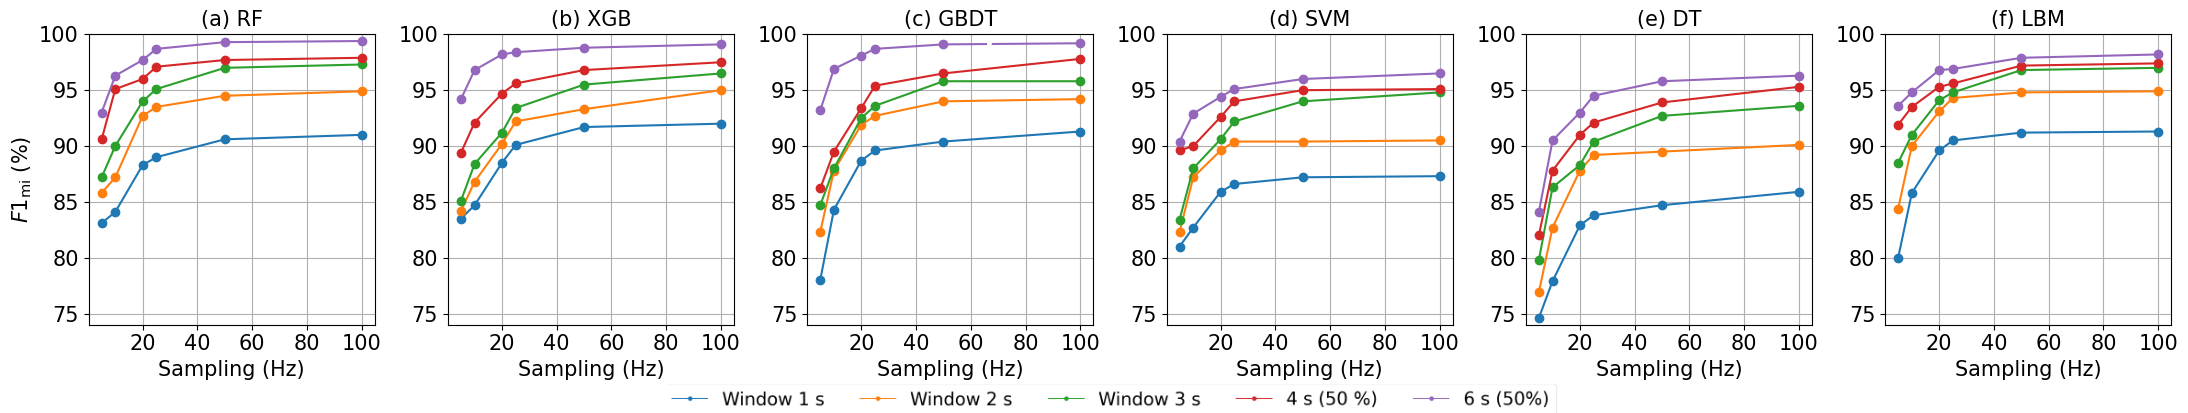
\includegraphics[width=1\linewidth,height=3.2 cm]{figure/accurracyonwindow.png}
\caption{$F1_{mi}$ of (a) RF, (b) XGB, (c) GBDT, (d) SVM, (e) DT, and (f) LBM, based on changes in $F_s$ and window size.} \label{accurracyonwindow}
\end{figure*}


The choice of window size and $F_s$ has a major influence on feature extraction and the optimization of ML performance \cite{frequency_window_2021}. This impact on the $F1_{mi}$ score is illustrated in Fig.~\ref{accurracyonwindow}, where six models were evaluated on the same private dataset. Experimental results show that the 6-second (overlap 50~\%) window, when applied to models, achieves stable and notable effectiveness across the entire $F_s$ range from 20 to 100~Hz. The models using the proposed feature set achieved $F1_{mi}$ scores above 95~\% when operating at sampling frequencies between 50~--~100~Hz with window sizes ranging from 3~--~6~s. While high performance was observed at 50~Hz, increasing the sampling rate to 100~Hz resulted in only marginal improvements, which were not significant considering the additional resource and energy consumption. For instance, RF, LBM, GBDT, DT, SVM, and XGB exhibited increases of only 0.2~--~0.3~\% when changing from 50~--~100~Hz, yet the maximum recognition performance could not be fully reached. A 6-second window yielded high performance, with $F1_{mi}$ scores above 99~\% (e.g., GBDT and LBM); however, reducing the window to 3 s led to a decrease of approximately 2~--~3~\%, and further shortening it to 1~s caused a more substantial drop of about 15~\%.

Although the 6-second window yielded $F1_{mi}$ above 99~\%, it posed a challenge for recognition of firefighter activities, where multiple actions often occur simultaneously within an observation. In contrast, shorter windows of 1 s and 2 s showed a significant performance reduction. The 3-second window showed a practical balance. Although its $F1_{mi}$ was approximately 2~--~3~\% lower than that of the 6-second window, it significantly mitigated the issue of overlapping actions in single observations and also reduced resource requirements for practical deployment. In addition, an $F_s$ of 50~Hz was found to be appropriate, as it reduced energy consumption compared to 100~Hz while still maintaining reliable recognition accuracy.


\subsection{Optimizing features}

Selecting features based on their importance has effectively reduced the number of features \cite{featureSelection2021,ImportandFeature2023}, computational complexity \cite{ViManhTuyen2024,HongNhung2023}, and model size, while maintaining high performance \cite{DaoHieu2022,Thu2022}. In this study, the combination of 13 feature types provides comprehensive insights into signal oscillation, symmetry, and stability, significantly enhancing the accuracy of action classification. Similarly, previous studies demonstrated that feature selection significantly impacted the accuracy of recognition models \cite{CHAI_FIRE2024,Lu2020,Wang2018}.

\begin{table}[h!]
\centering
\caption{Comparison of feature effectiveness on the private dataset.}
\label{table_changefeature}
\resizebox{\columnwidth}{!}{ % Co bảng theo chiều rộng của cột
    \begin{tabular}{
        >{\arraybackslash}m{0.5\linewidth}
        >{\arraybackslash}m{0.2\linewidth}
        >{\arraybackslash}m{0.18\linewidth}
        }
\noalign{\hrule height 1.2pt} % Dòng kẻ tiêu đề đậm hơn
\rowcolor{gray!20}\textbf{Applied features} & \textbf{Feature types} & \textbf{$F1_{mi}$~(\%)}  \\

\noalign{\hrule height 1.2pt} % Dòng kẻ tiêu đề đậm hơn
Proposed & 13 & \textbf{96.1} \\

Remove energy  & 12 & 93.4 ($\downarrow$2.7)\\

Remove mean absolute deviation & 12 & 93.5 ($\downarrow$2.6) \\

Remove signal magnitude area. & 12 & 93.3 ($\downarrow$2.8)  \\

Remove average amplitude change & 12 & 93.0 ($\downarrow$3.1)   \\

Remove simple square integral  & 12 & 93.8 ($\downarrow$2.3) \\

Remove mean & 12 & 92.6 ($\downarrow$3.5)\\

Remove standard deviation & 12 & 93.0 ($\downarrow$3.1) \\

Remove maximum & 12  & 93.0 ($\downarrow$3.1) \\

Remove interquartile range & 12 & 93.6 ($\downarrow$2.5)  \\

Remove hjorth complexity & 12  & 93.0 ($\downarrow$3.1) \\

Remove median absolute deviation & 12 & 93.8 ($\downarrow$2.3) \\

Remove range & 12 & 93.2 ($\downarrow$2.9) \\
\hline

Chai \cite{CHAI_FIRE2024} proposed 20 time and 6 frequency domain feature types & 26 & 95.6 ($\downarrow$0.6)\\
\hline
Wang \cite{Wang2018} proposed 11 time and 2 frequency domain feature types & 16 & 92.9 ($\downarrow$3.2)  \\
\hline
Vi \cite{ViManhTuyen2024} proposed average absolute deviation, std, iqr, range, and energy  & 5 & 85.7 ($\downarrow$10.4) \\
\hline
Hong \cite{HongNhung2023} proposed mean, std, median, range,  energy & 5 & 83.1 ($\downarrow$13)\\

% \hline
\noalign{\hrule height 1.2pt} % Dòng kẻ tiêu đề đậm hơn
\end{tabular}

}
\end{table} 


 Tab.~\ref{table_changefeature} compares the $F1_{mi}$ performance when modifying the proposed feature set. Adjusting the number of features compared to the proposed feature set has resulted in poorer performance. When the full set of proposed features (13 features) was applied, the model achieved $F1_{mi}=96.1~\%$, which was the highest among all cases. When individual feature types were removed, $F1_{mi}$ decreased in all cases, indicating that each feature contributed to the recognition performance. In particular, removing features such as energy, mean absolute deviation, or signal magnitude area led to more noticeable drops in performance, with $F1_{mi}$ reduced to 93.4~\%,93.5~\%, and 93.3~\%, respectively. For feature sets with larger numbers of features, such as Chai's set of 26 feature types \cite{CHAI_FIRE2024}, an $F1_{mi}$ of 95.6~\% was achieved, while Wang's 16 feature types \cite{Wang2018} reached $92.9~\%$. In contrast, feature sets with fewer features, such as those proposed by Vi \cite{ViManhTuyen2024} and Hong \cite{HongNhung2023}, resulted in lower performance, with $F1_{mi}$ values of $85.7~\%$ and $83.1~\%$, respectively. Therefore, the proposed feature set offers a good balance between feature quantity and recognition performance. 
 
 In general, the proposed feature set contains comprehensive information, achieving a balance between classification performance and computational complexity, making it suitable for the specific requirements of firefighter action recognition. While other feature sets may reduce the number of features or increase the processing speed, they fail to compensate for the loss of critical information when certain features are removed. In the context of prolonged rescue operations, increasing the number of features results in higher computational time, negatively affecting recognition performance when processing real-time data, while the improvement in accuracy is negligible, or accuracy may even decrease. 
 
\subsection{Limitation and feature work}


Although the proposed system has many advantages, several limitations need to be addressed to enhance its practical applicability. Firstly, the system has a large size due to its manually assembled design, which causes inconvenience during field deployment. Optimizing its size and design for easy integration with support equipment such as clothing and belts is essential. A further limitation is that the system was developed and evaluated primarily using data from male volunteers with body types closely resembling those of professional firefighters. While this sampling strategy aligns with the system’s intended application, it may limit the model’s adaptability to firefighters with substantially different physical characteristics, such as female personnel or those with atypical body builds.

Additionally, the current system is only a small part of the overall positioning system and has not yet incorporated critical features such as location tracking and emergency alerts. Adding these features will improve usability and facilitate timely information transmission to commanders. However, the integration process requires close coordination among software, hardware, and data transmission protocols, necessitating additional time and resources for development. Optimizing the system's size, weight, and hardware upgrades will be a key objective to provide a more comprehensive and effective solution for firefighters in emergency situations. 

In the future, the research aims to develop a comprehensive emergency support system that includes monitoring work status, issuing emergency alerts in hazardous situations, and creating a support network for multiple firefighters simultaneously.
\section{Conclusion}\label{Conclusion}

This study constructed a dedicated dataset simulating firefighter rescue activities to supplement existing public datasets, and developed a signal processing pipeline that combines a sliding window technique and abnormality index to improve the recognition of transition actions. As a result, the position and starting time of the sliding window are adjusted appropriately to fully capture an action. Based on this foundation, the RFAR system, which employs a lightweight wearable device and an optimized RF model, was implemented on a low-power microcontroller. The system achieved an $F1_{mi}$ of over 96~\% in private dataset and over 78~\% on three public datasets. The system operated effectively on real-time accelerometer data from volunteers wearing the device during rescue drills, with all metrics exceeding 96~\%. In terms of practical applications, the proposed system is highly applicable and serves as a vital component of an indoor emergency positioning support system for firefighters.

\section*{Acknowledgment}
This study was funded by project code MHN2024-01.02 from the Hanoi Open University.

\section*{Appendix}\label{Appendix}
Demo video showcasing the research: https://youtu.be/S4hAzgEo-NA

Source code: https://github.com/HieuSSALAB/FireFighter
\section*{Declarations}\label{Declarations}
\textbf{Ethics approval}. This study was approved by The Ethical Review Board for Biomedical Research of Phenikaa University (number: 024.22/DHP-HDDD). All procedures involving human participants adhered to the ethical standards of the research committee and the 1964 Helsinki Declaration along with its subsequent amendments.\\

\textbf{Data availability}. Dataset in this research was collected by the authors and volunteers, fully complying with privacy and ethical regulations. Scientists wishing to use the data must cite this paper and acknowledge the source.
Link: https://dx.doi.org/10.21227/9w3p-v638
\bibliographystyle{IEEEtran}
\bibliography{sn-bibliography}% common 

% \begin{IEEEbiography}[{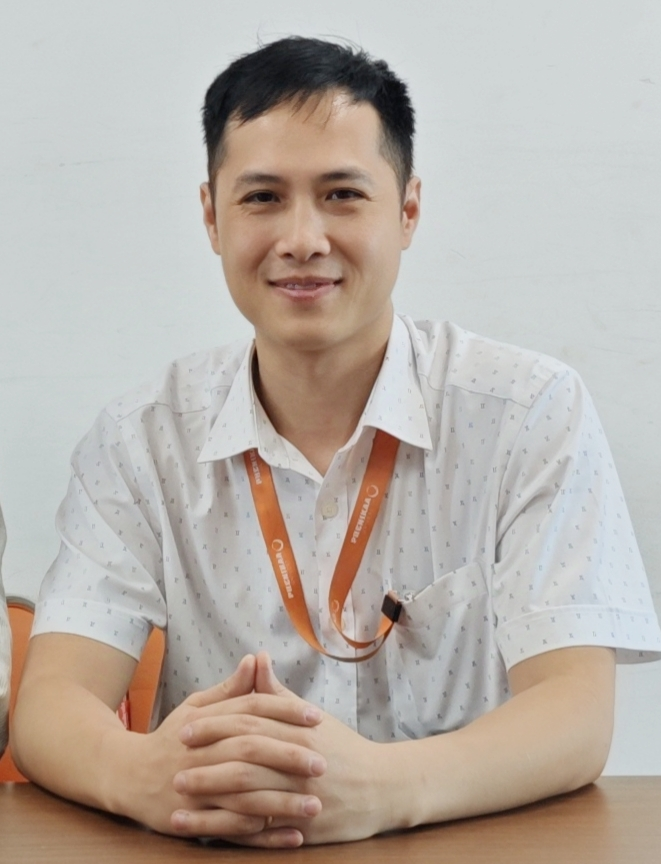
\includegraphics[width=1in,height=1.25in,clip,keepaspectratio]{avatar/DaoToHieu.jpg}}]{To-Hieu Dao} is a Master at Phenikaa University. He has conducted approximately 12 institutional-level scientific research projects and supervised many studentlevel research projects. In 2019 and 2021, he received commendation certificates from the Director of Thai Nguyen University. In 2022, he was honored to receive a commendation certificate from the Minister of Education and Training. From 2022-2024, he received a commendation certificate from the President of Phenikaa University.
% \end{IEEEbiography}

% \begin{IEEEbiography}
% [{
\includegraphics[width=1in,height=1.2in,clip,keepaspectratio]{avatar/tdn.png}}]{Duc-Nghia Tran} is a PhD at the Institute of Information Technology, Vietnam Academy of Science and Technology (VAST). He received his PhD degree from Sorbonne Paris Cite´ (France). In his thesis, he focuses on signal processing of EPR spectra for in vivo experiments. His research interests are AI, IoT, Electron Paramagnetic Resonance, parameter estimation, and data analysis. He serves as a technical committee program member and reviewer of many international conferences and journals.
% \end{IEEEbiography}

% \begin{IEEEbiography}[{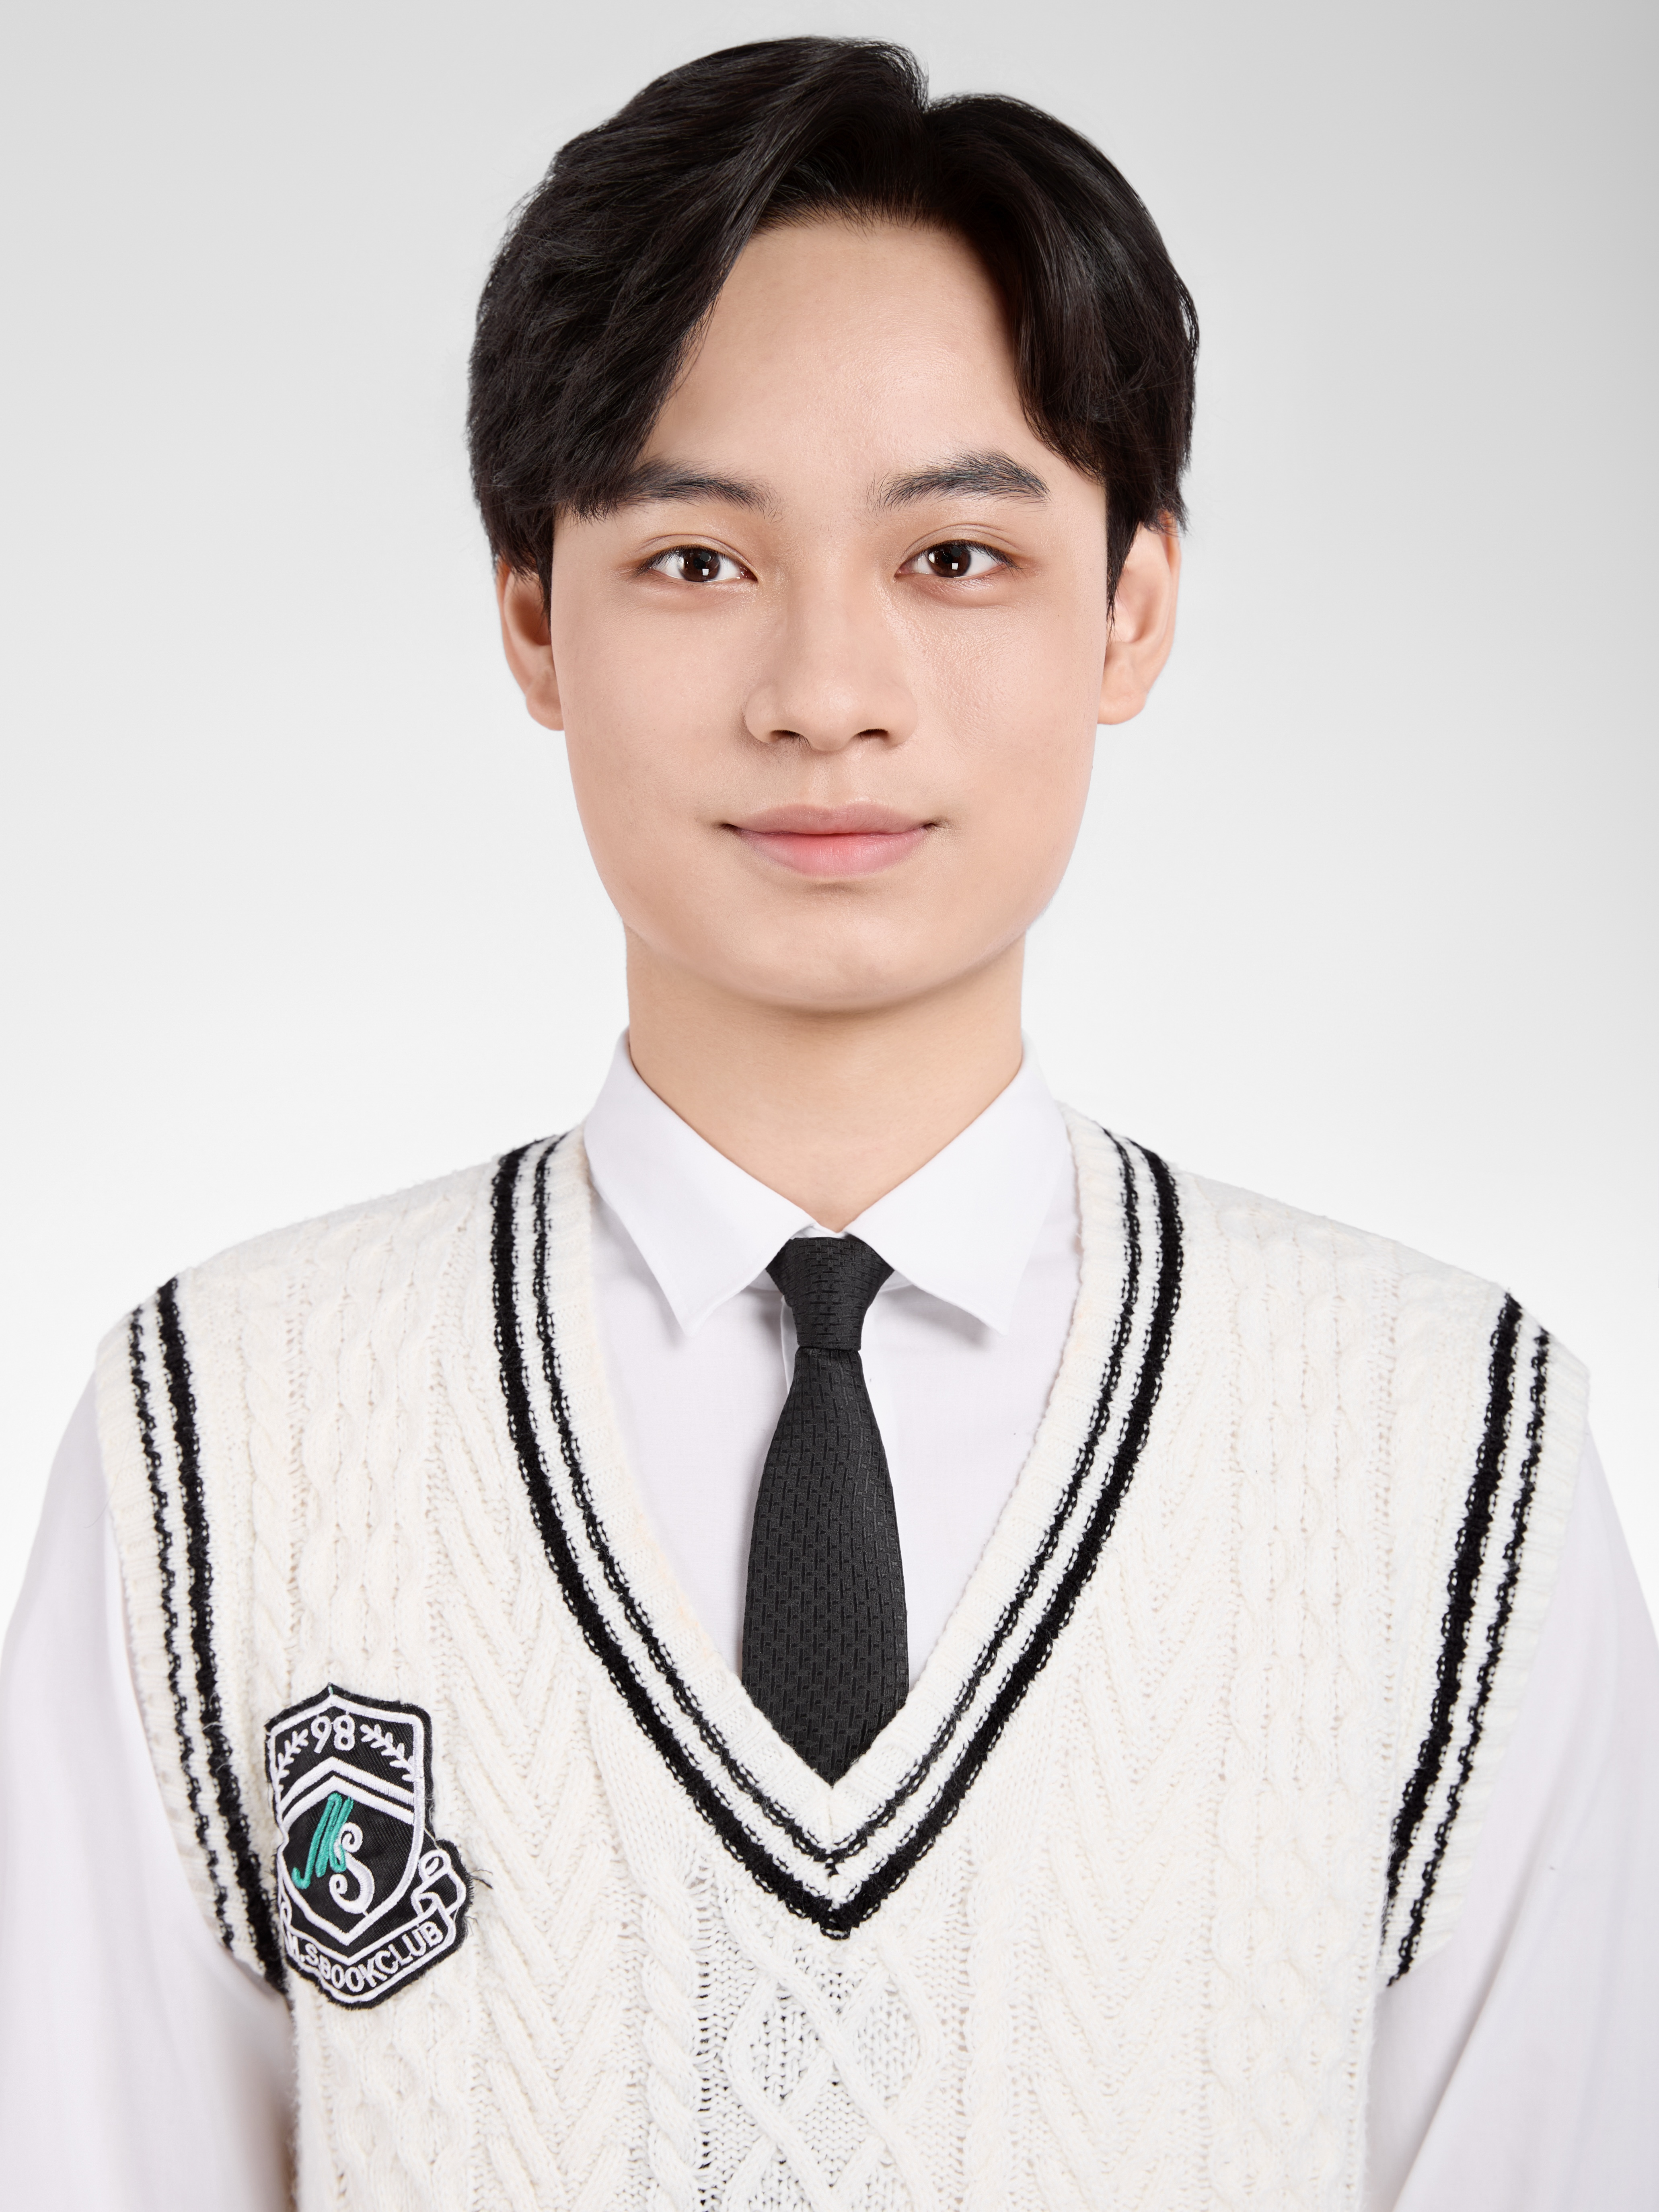
\includegraphics[width=1in,height=1.25in,clip,keepaspectratio]{avatar/bvh.png}}]{Viet-Hoan Bui} is a dedicated Biomedical Engineering undergraduate at Phenikaa University. His academic journey is distinguished by several notable achievements, including first prizes in scientific research at Phenikaa University and prestigious awards in national competitions such as the "Science and Technology Awards for Students in Higher Education Institutions." His work encompasses integrated sensors, machine learning, and advanced signal processing for healthcare applications.
% \end{IEEEbiography}

% \begin{IEEEbiography}[{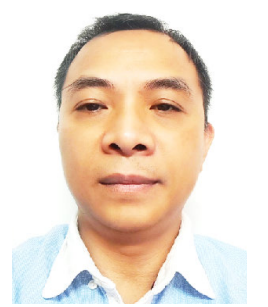
\includegraphics[width=1in,height=1.3in,clip,keepaspectratio]{avatar/nvson.png}}]{Van Son Nguyen} received a B.E. degree in Electrical Engineering and an M.S. degree in Electronics and Telecommunications Engineering from Hanoi Open University, Vietnam. He is currently a Lecturer with the Faculty of Electrical and Electronic Engineering, at Hanoi Open University. His research interests include signal processing in B5G/6G systems and ML/AI applications in big data processing.
% \end{IEEEbiography}

% \begin{IEEEbiography}[{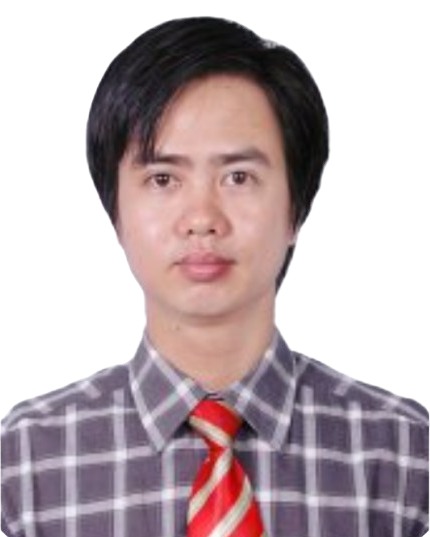
\includegraphics[width=1in,height=1.3in,clip,keepaspectratio]{avatar/dkhoa.png}}]{Dang Khanh Hoa} graduated from Hanoi University of Science and Technology in 2002, majoring in Electronics and Telecommunications. In 2005, he graduated with a master’s degree in Electronic Engineering from Hanoi University of Science and Technology. In 2020, he was awarded a doctorate in Electronic Engineering at the School of Electrical and Electronics Engineering, Hanoi University of Science and Technology. His research focuses mainly on computer vision, applied to wheeled robot control.
% \end{IEEEbiography}

% \begin{IEEEbiography}[{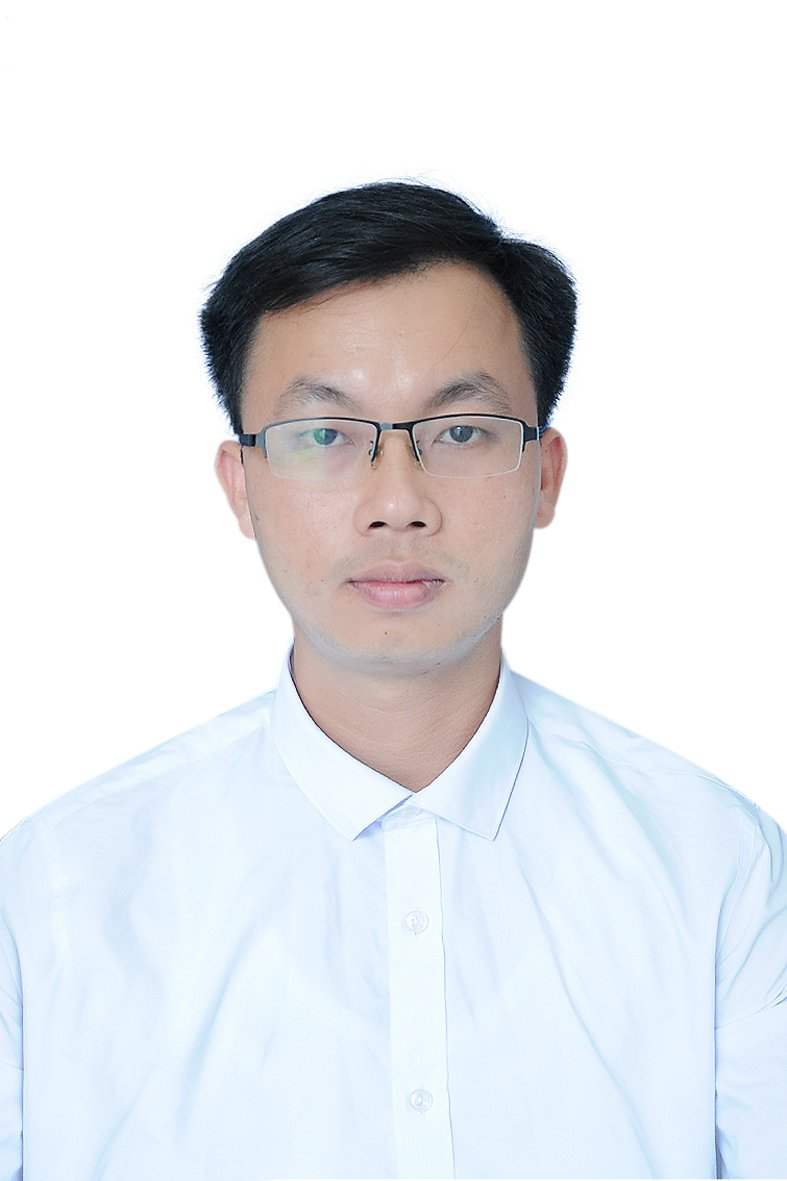
\includegraphics[width=1in,height=1.3in,clip,keepaspectratio]{avatar/pvt.jpg}}]{Pham Van Thanh}  was born in 1990. He received the M.Sc. degree in Electronics and Telecommunication at University of Engineering and Technology in 2012 and he was a PhD student at this university. He also is a full-time lecturer at University of Fire Prevention and Fighting.  His research interest covers areas that include Signal and Image Processing, Personal Safety Equipment, Firefighter Supporting Devices, and Fire Protection Systems. He successfully defended his doctoral thesis in 2022.
% \end{IEEEbiography}

% \begin{IEEEbiography}[{
\includegraphics[width=1in,height=1.25in,clip,keepaspectratio]{avatar/tdt.jpg}}]{Duc-Tan Tran} is a Professor and Vice Dean of the Faculty of Electrical and Electronic Engineering, at Phenikaa University. He has published over 150 research papers. His main research interests include the representation, processing, analysis, and communication of information embedded in signals and datasets. He serves as a TP Co-chair, technical committee program member, track chair, session chair, and reviewer of many international conferences and journals.
% \end{IEEEbiography}

% \begin{figure*}[p] % 'p' đặt hình ảnh vào trang riêng
% \centering
% 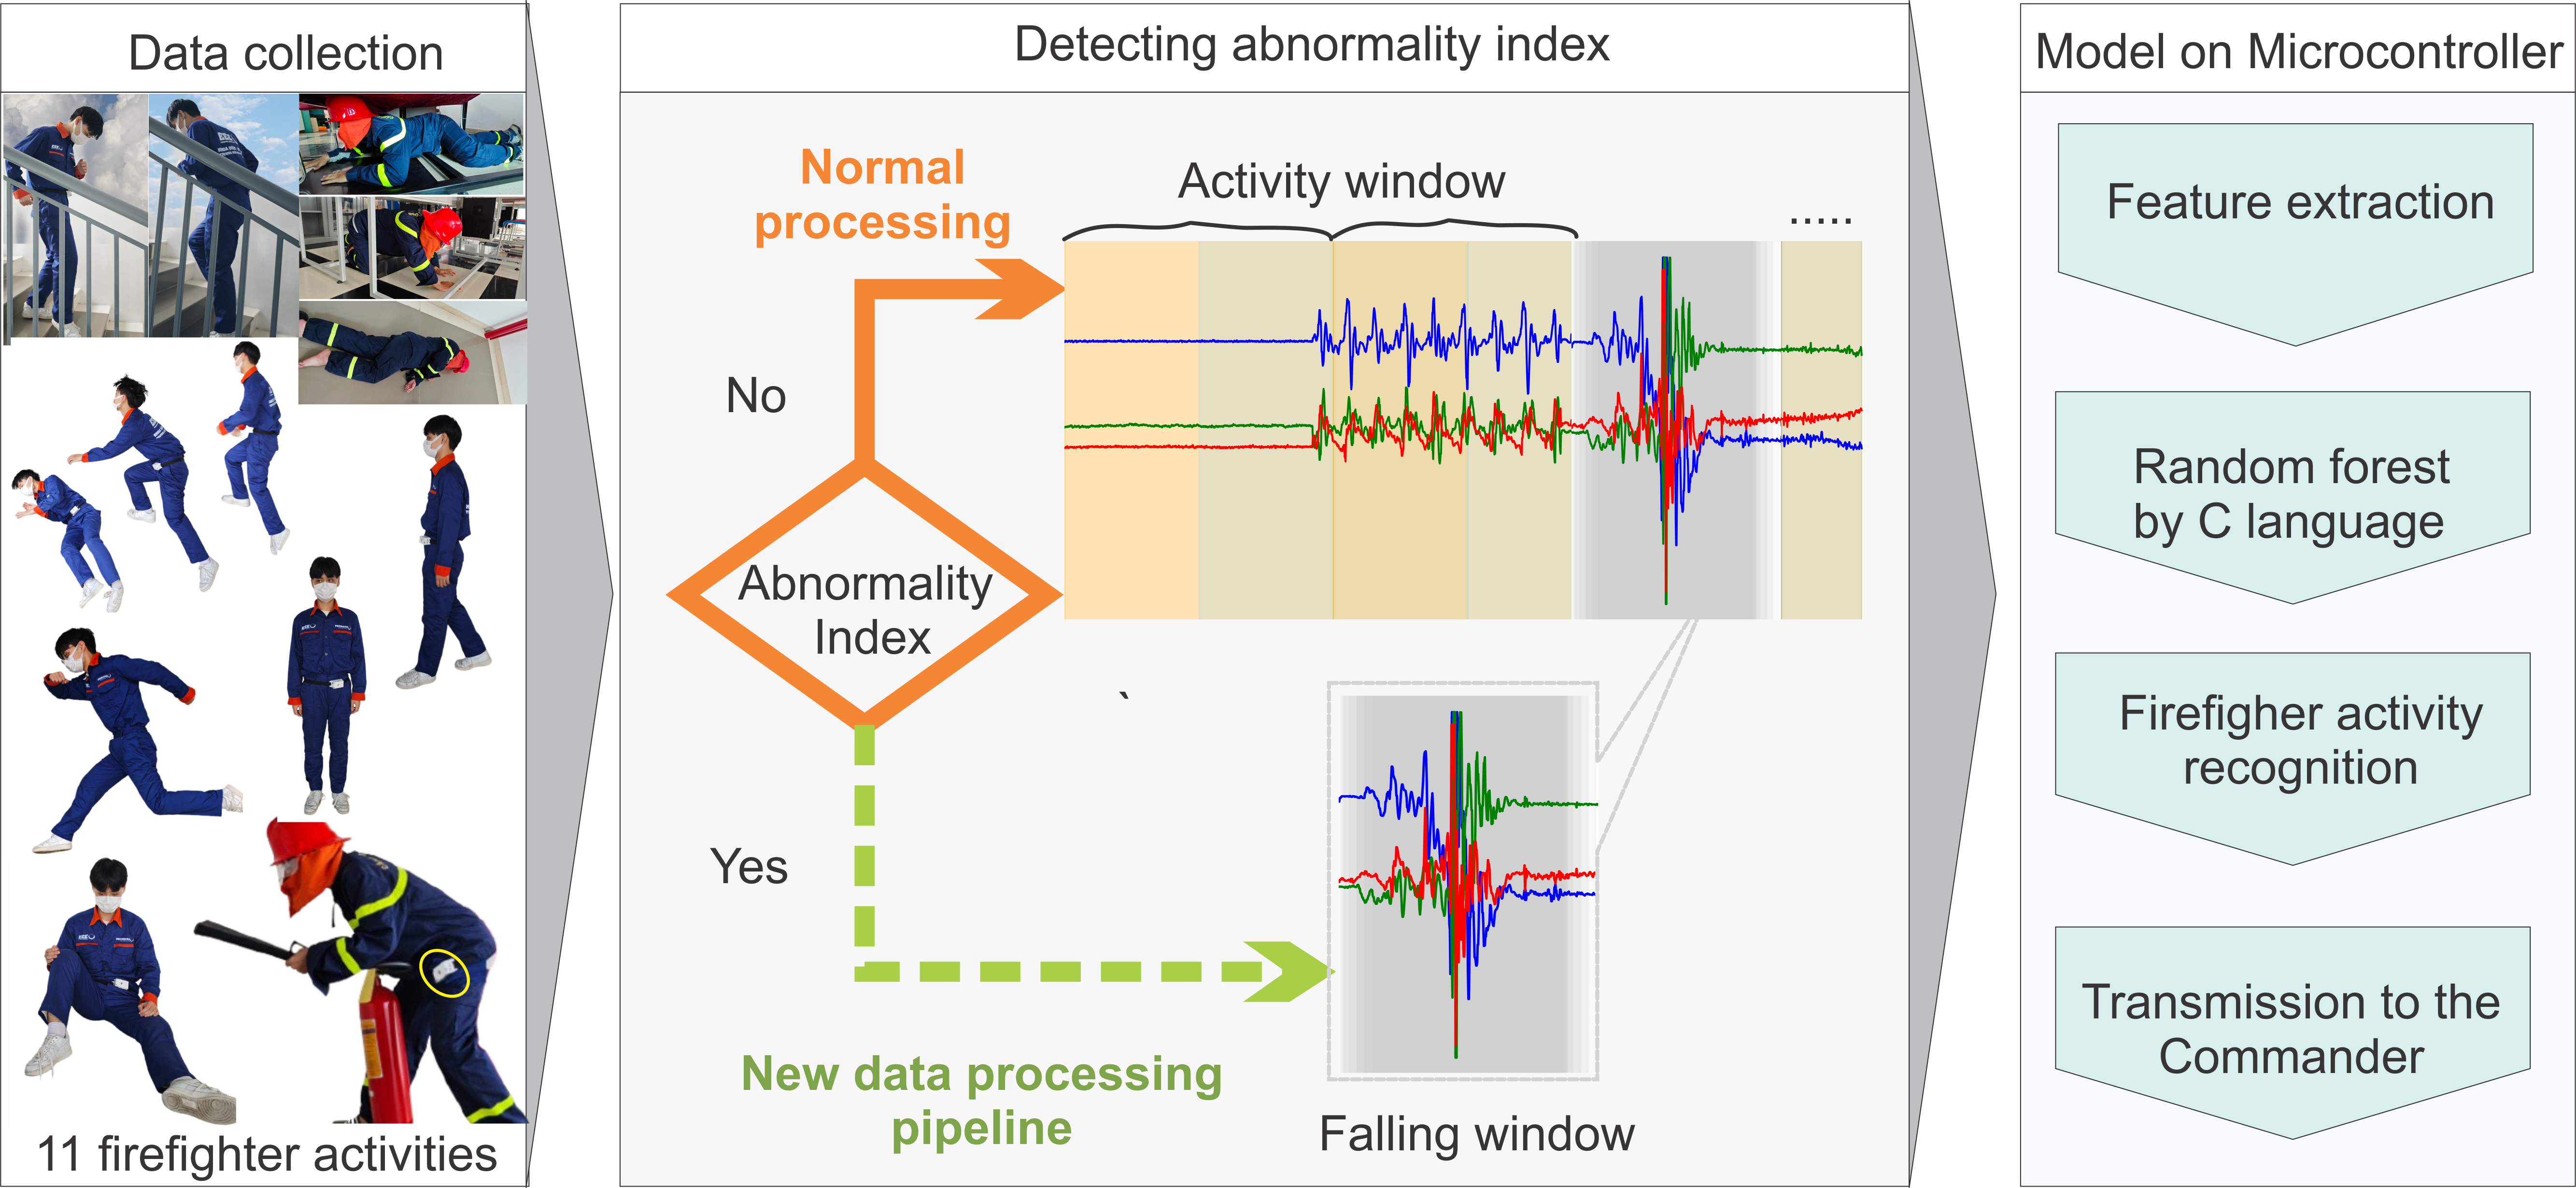
\includegraphics[width=1.36\linewidth, angle=270]{figure/graph linh cuu hoa.png} 
% \end{figure*}

\end{document}
